%% Copernicus Publications Manuscript Preparation Template for LaTeX Submissions
%DIF LATEXDIFF DIFFERENCE FILE
%DIF DEL version_2/acp-2017-34-manuscript-version2.tex   Wed Jul 26 14:40:31 2017
%DIF ADD vsls_emissions.tex                              Thu Aug 10 13:53:28 2017
%% ---------------------------------
%% This template should be used for copernicus.cls
%% The class file and some style files are bundled in the Copernicus Latex Package, which can be downloaded from the different journal webpages.
%% For further assistance please contact Copernicus Publications at: production@copernicus.org
%% http://publications.copernicus.org/for_authors/manuscript_preparation.html


%% Please use the following documentclass and journal abbreviations for discussion papers and final revised papers.


%% 2-column papers and discussion papers
\documentclass[acp, manuscript]{copernicus}

%% Journal abbreviations (please use the same for discussion papers and final revised papers)

% Archives Animal Breeding (aab)
% Atmospheric Chemistry and Physics (acp)
% Advances in Geosciences (adgeo)
% Advances in Statistical Climatology, Meteorology and Oceanography (ascmo)
% Annales Geophysicae (angeo)
% ASTRA Proceedings (ap)
% Atmospheric Measurement Techniques (amt)
% Advances in Radio Science (ars)
% Advances in Science and Research (asr)
% Biogeosciences (bg)
% Climate of the Past (cp)
% Drinking Water Engineering and Science (dwes)
% Earth System Dynamics (esd)
% Earth Surface Dynamics (esurf)
% Earth System Science Data (essd)
% Fossil Record (fr)
% Geographica Helvetica (gh)
% Geoscientific Instrumentation, Methods and Data Systems (gi)
% Geoscientific Model Development (gmd)
% Geothermal Energy Science (gtes)
% Hydrology and Earth System Sciences (hess)
% History of Geo- and Space Sciences (hgss)
% Journal of Sensors and Sensor Systems (jsss)
% Mechanical Sciences (ms)
% Natural Hazards and Earth System Sciences (nhess)
% Nonlinear Processes in Geophysics (npg)
% Ocean Science (os)
% Proceedings of the International Association of Hydrological Sciences (piahs)
% Primate Biology (pb)
% Scientific Drilling (sd)
% SOIL (soil)
% Solid Earth (se)
% The Cryosphere (tc)
% Web Ecology (we)
% Wind Energy Science (wes)

%% \usepackage commands included in the copernicus.cls:
%\usepackage[german, english]{babel}
%\usepackage{tabularx}
%\usepackage{cancel}
%\usepackage{multirow}
%\usepackage{supertabular}
%\usepackage{algorithmic}
%\usepackage{algorithm}
%\usepackage{amsthm}
%\usepackage{float}
%\usepackage{subfig}
%\usepackage{rotating}
%DIF PREAMBLE EXTENSION ADDED BY LATEXDIFF
%DIF UNDERLINE PREAMBLE %DIF PREAMBLE
\RequirePackage[normalem]{ulem} %DIF PREAMBLE
\RequirePackage{color}\definecolor{RED}{rgb}{1,0,0}\definecolor{BLUE}{rgb}{0,0,1} %DIF PREAMBLE
\providecommand{\DIFadd}[1]{{\protect\color{blue}\uwave{#1}}} %DIF PREAMBLE
\providecommand{\DIFdel}[1]{{\protect\color{red}\sout{#1}}}                      %DIF PREAMBLE
%DIF SAFE PREAMBLE %DIF PREAMBLE
\providecommand{\DIFaddbegin}{} %DIF PREAMBLE
\providecommand{\DIFaddend}{} %DIF PREAMBLE
\providecommand{\DIFdelbegin}{} %DIF PREAMBLE
\providecommand{\DIFdelend}{} %DIF PREAMBLE
%DIF FLOATSAFE PREAMBLE %DIF PREAMBLE
\providecommand{\DIFaddFL}[1]{\DIFadd{#1}} %DIF PREAMBLE
\providecommand{\DIFdelFL}[1]{\DIFdel{#1}} %DIF PREAMBLE
\providecommand{\DIFaddbeginFL}{} %DIF PREAMBLE
\providecommand{\DIFaddendFL}{} %DIF PREAMBLE
\providecommand{\DIFdelbeginFL}{} %DIF PREAMBLE
\providecommand{\DIFdelendFL}{} %DIF PREAMBLE
%DIF END PREAMBLE EXTENSION ADDED BY LATEXDIFF

\begin{document}
% Authors' response
\thispagestyle{empty}
\section*{Authors' response}
\subsection*{{\color{blue}acp-2017-34-RC1-supplement (31 March 2017)}}
The authors thank the anonymous referee \#2 for his constructive comments regarding our paper. We will answer his/her specific questions in detail in the following. Accordingly, we will provide comprehensive discussions and additional numbers in a revised version of the paper where further clarifications are needed.
\begin{itemize}
\item Specific comments:
  \begin{itemize}
  \item[$\bullet$]{\color{blue}Sensitivity of VSLS emissions wrt. water concentrations/wind/SST:} No simulation study has been conducted in the regard of changing water concentrations of VSLS \emph{and} a change in climate. Therefore no assessment can be made. At present, global mean \chem{CH_2Br_2}/\chem{CHBr_3} concentrations in ocean water are close to equilibrium with atmospheric concentrations which is causing a high sensitivity of ocean--atmosphere fluxes to changes in the atmosphere~\citep{ACP:Lennartz2015}. There are different potential future scenarios. The current scenario could be interpreted as an increase in production in response to increased fluxes to compensate a detrainment. Increased fluxes and decreasing production at the same time may lead to decreasing concentrations and in turn decreasing fluxes. Regarding a dependence of VSLS fluxes wrt. SSTs and wind, our data show a strong correlation between VSLS fluxes and former ($\Phi_\text{VSLS}(\text{SST})\propto \text{SST}$), but a much weaker (or even anti-) correlation to latter.
  \item[$\bullet$]{\color{blue}Emission perturbation's influence on ozone:} Unfortunately, our long-term simulations do not allow for an assessment of ozone changes induced through VSLS emission perturbations. SC\_free does not include interactive ozone chemistry, whereas RC2-base-05 incorporates prescribed fluxes based on scenario five by~\citet{JGR:Warwick2006}.
  \item[$\bullet$]{\color{blue}Chlorine moderation of bromine influence on ozone:} Future projections of stratospheric chlorine loading are shown, e.g., in~\citet[][Chap. 12]{IPCC2013} or~\citet[][Chap.2]{WMO2014}. Stratospheric \chem{Cl_y} peaks in 2000. Assuming an adherence to the Montreal protocol, stratospheric volume mixing ratios of \chem{Cl_y} will decay exponentially in the course of the 21st century. From \citet[][Chap.2, Fig. 2--21]{WMO2014}, a decrease of \chem{Cl_y} loading at 1\,\unit{hPa} of about 2\,\unit{ppbv} between 2000 and 2080 can be deduced. We will provide numbers of peak and end of 21st century values for the \chem{Cl_y} load in the stratosphere in accordance to our simulations. We acknowledge, the combined effect of chlorine and bromine is not negligible. However, it can not be assessed with our simulations. RC2-base-05 is not accompanied by a sensitivity study with no VSLS emission. RT1a/RT1b have the same chlorine load and do not include present day. The moderation of differing chlorine loading on bromine influence on ozone has been studied in detail by \citet{ACP:Yang2014} and \citet{GRL:Sinnhuber2015}. \citet{ACP:Yang2014} show for two stratospheric \chem{Cl_y} loadings (3\,\unit{ppb}, 0.8\,\unit{ppb}) corresponding to 2000 and 2100 values and differing VSLS contribution to stratospheric bromine loading, the more chlorine the stronger ozone is affected by increasing bromine mixing ratios from VSLS. Between the two \chem{Cl_y} scenarios a $\Delta$\chem{O_3} of about 0.5--0.6\,\unit{ppmv} (80$^\circ$ S) and 0.3--0.4\,\unit{ppmv} (80$^\circ$ N) has been found. 
  \item[]{\color{blue}P1 L1:} The sentence has been changed in accordance to the comment: \emph{Very short-lived substances~(VSLS) contribute as source gases [...]}
  \item[]{\color{blue}P2 L4:} Accordingly, the acronym definition has been changed and moved to the proper sentence: \emph{Minor brominated very short-lived substances (VSLS) include [...]. The tropospheric lifetime of these gases lies between several days to weeks.}
  \item[]{\color{blue}P2 L6--7:} The definitions at this point have been removed since they are, indeed, redefined later on.
  \item[]{\color{blue}P5 L12--15:} In accordance to the comments a specification of temperature and transfer velocities has been added: \emph{The transfer velocity depends largely on temperature $T_\text{air}$ and surface wind speed which is taken into account by distinguishing between water- and air-side transport velocities ($k_\text{w}$, $k_\text{air}$).}
  \end{itemize}
\end{itemize}
\newpage
%
\subsection*{{\color{blue}acp-2017-34-RC1-supplement (18 Jul 2017)}}
The authors thank the anonymous referee \#1 for his/her thorough work and stimulating comments regarding our paper. Detailed response to the posed questions will be given in the following.
\begin{itemize}
\item Major comments:
\begin{itemize}
\item[1.]{\color{blue}There is a notorious omission to a strongly related paper from \citet{JAC:Ziska2017}, which used exactly the same methodology to address the future evolution of the ocean-atmosphere flux of VSL through the 21st century. Even when the current study goes beyond the above-mentioned work by addressing the atmospheric factors controlling the VSL stratospheric injection and impact on ozone, a comparison and description of the similarities and differences regarding the \citet{JAC:Ziska2017} paper should be given.}
  We have include a discussion of the \citet{JAC:Ziska2017} results and how they relate to our work. \citet{JAC:Ziska2017} was published online on 29 December 2016, only a few days before our submission.
  \begin{itemize}
  \item[$\bullet$]{\color{blue} Ziska et al. considered the RCP 2.6 and RCP 8.5 scenarios, and determined a linear response only for the 1979--2005 period, but not when projecting into the future. Additionally, their RCP 2.6 increase of brominated emissions (9\%) is of the same magnitude as the one found here for RCP 6.0 (10\%).}
    There is a fundamental difference between the Ziska approach an ours: \citet{JAC:Ziska2017} diagnosed the flux from parameters such as SST and wind speed for a fixed concentration gradient. In our work, we compute the flux, consistently, i.e. based on changing atmospheric concentrations under the assumption of a prescribed ocean water concentration. From a theoretical point of view it is clear that we will compute a smaller increase in flux with our approach.
  \item[$\bullet$]{\color{blue} P3 L3: ``In these simulations, \chem{OH} concentrations have been set to zero in the lower troposphere (700–-1000 hPa) to reduce the variability of ground level volume mixing ratio (VMR) of VSLS''. Thus, degradation of \chem{CHBr_3} and mostly \chem{CH_2Br_2} in the MBL and Lower troposphere is not well represented and might affect their tropospheric concentration ($C_\mathrm{air}$). But eq. 1, which infers the future evolution of VSLS emissions, depends on the $C_\mathrm{air}$ concentration, which would be larger than if \chem{OH} values would have not been forced to zero in the MBL. Could this assumed configuration be related to the similar \% between RCP 2.6 from \citet{JAC:Ziska2017} and present work?}
    First: \chem{OH} was set to zero in the MBL only in the simulations SC\_free and SC\_nudged, not in any of the others. It is true that we overestimate the chemical lifetime of the VSLS in the MBL and that a shorter lifetime may result in a stronger flux and stronger flux increase depending on the future scenario. We will include this caveat in our revised manuscript: \emph{Only in these simulations with simplified chemistry, \chem{OH} concentrations have been set to zero in the lower troposphere [...]. The chemical lifetime of VSLS in the lower troposphere is therefore overestimated. Due to the longer lifetime, VSLS are more abundant in the lower troposphere leading to a flux suppression.}
  \end{itemize}
\item[2.]{\color{blue}Consideration of heterogeneous recycling of \chem{Br_y^{VSL}} in the UT and TTL might be of major importance in current study, and there is not a single mention of it neither in the model configuration nor in the results analysis. Many modelling studies, including some performed by the same group \citep{ACP:Aschmann2009}, other cited in the text \citep{ACP:Liang2014} and many others not even mentioned in the manuscript (Parrella et al., 2012; Fernandez et al., 2014; Wang et al., 2015; Schmidt et al., 2016) highlight the importance of considering heterogeneous recycling occurring on ice-crystals and sea-salt aerosols as they can increase the lifetime against wet-removal or represent an additional source of bromine to the troposphere, respectively. Indeed, Fig. 5 and Fig. 9 clearly shows that \chem{Br_y^{VSLS}} is the dominant fraction controlling the total stratospheric \chem{Br_{Tot}^{VSLS}} change between present time and 2100, which highlight the importance of properly representing inorganic product gases chemistry in present study.}
  There is, in fact, multiple evidence that heterogeneous reactions converting soluble \chem{HBr} and \chem{HOBr} into insoluble \chem{BrO} may play a role. We did not explicitly test these mechanisms in our model simulations. We will include a discussion of the possible implications in our revised manuscript and are grateful for comments and suggested further references.
  \begin{itemize}
  \item[$\bullet$]{\color{blue}Authors should decide whether performing additional simulations including and neglecting the heterogeneous recycling reactions is necessary or not. But if they instead want to focus on VSL source gases, at least the paper must mention how the uncertainties of heterogeneous recycling processes could be affecting their overall stratospheric results. A very rapid analysis could indicate that because of the increased tropospheric degradation, there is a larger \chem{Br_y} fraction that is effectively washed out from the troposphere and never reaches the stratosphere. Thus, reducing the overall PG stratospheric injection. If that is the case, then it should be explicitly mentioned in the text, supported with more details about the deposition efficiencies of \chem{Br_y} species.}
    First, we would like to stress that the increase of lower stratospheric VSLS in the future due to enhanced upwelling is counteracted by a corresponding decrease in inorganic bromine. Everything else unchanged, an increase in upwelling will not change the total bromine in the stratosphere. In addition to this, we do find a future decrease in total bromine due to VSLS and part of this is due to the reduced lifetime of VSLS in the troposphere because of increased \chem{OH} reactivity. We do, however, acknowledge that there are still structural uncertainties on the recycling of \chem{Br_y} in the troposphere, which may have an impact on the washout (and there are also structural uncertainties in the treatment of washout itself). We will address this caveat in the revised manuscript.
  \item[$\bullet$]{\color{blue}Abstract, P1 L7: ``A decrease in the tropospheric mixing ratios of VSLS and an increase in the lower stratosphere are attributed to changes in atmospheric chemistry and transport. Our model simulations reveal that, in line with the reduction in the troposphere, the total amount of bromine from VSLS in the stratosphere will decrease during the 21st century''. I found a contradiction between these two sentences included in the abstract, which is not clarified nor consistent with the final sentence in Section. 4.2}
    Yes, these sentences are not fully consistent. We rewrite this to make our point clear: \emph{Our model simulations reveal that this increase is counteracted by a corresponding reduction of inorganic bromine. Therefore the total amount of bromine from VSLS in the stratosphere will not be changed by an increase in upwelling.}
  \item[$\bullet$]{\color{blue}Section 4.2, P13 L15: ``To summarize, the main reason to the apparent increase of bromine from VSLS above 100 hPa in RC2-base-05 of about 5–10\% is the increase in vertical transport in the tropics. Although bromine loading from VSLS above 100 hPa is increased at the end of the 21st century, the stratospheric abundance of bromine from VSLS is not increasing but decreasing by about 1–2 ppt, if an upward shift of the tropopause is taken into consideration.'' This summarizing result seems not to be consistent with the rest of the text nor what is shown in the figures. The only 1-2 ppt reduction occurs in \chem{Br_y} PG (Fig. 9a, center), which as I have mentioned above, might not be well represented in the modeling study and might be altering the interpretation of the results. Additionally, the 1-2 ppt difference appears for $\Delta P > 20$ hPa respect the tropopause, so changes in the tropopause height could be affecting the VSLS \chem{Br_y} levels in the UTLS, but not in the stratospheric over-world.}
    Yes, the final sentences in Section~4.2 (P13 L15) are not fully consistent with the abstract. We rewrite this accordingly: \emph{[...] the increase of lower stratospheric VSLS in RC2-base-05 of about 5--10\% is due to enhanced vertical transport in the tropics. This increase is, however, counteracted by a corresponding decrease in inorganic bromine. Everything else unchanged, an increase in tropical upwelling will therefore not change the total amount of bromine in the future stratosphere. Additionally, due to enhanced future \chem{OH} concentrations in RCP6.0, the tropospheric lifetime of VSLS is reduced which leads to a decrease of total bromine from VSLS. In this case, as mentioned in Section~\ref{sec:emission_trends}, whether the amount of inorganic PG in the UTLS is decreasing or not, strongly depends on the partitioning of \chem{Br_y} and conversation of soluble \chem{HBr} and \chem{HOBr} into insoluble \chem{BrO} through heterogeneous recycling, e.g., occurring on sea-salt aerosols or ice-crystals. In case insoluble species are favored, vertical transport would enhance the amount of PG in the UTLS. Otherwise, wet removal in the troposphere would decrease the amount of PG. This mechanism has not been explicitly tested in our model simulations.}
  \item[$\bullet$]{\color{blue}Forcing \chem{OH} to be zero in the LT also reduces the total amount of inorganic bromine product gas species being available for heterogeneous recycling. This could reduce the additional source from sea-salt dehalogenation (if considered). How this forced \chem{OH} assumption could be affecting the treatment of the PG being released from aerosols?}
     \chem{OH} is set to zero only in the SC\_free and SC\_nudged simulations in Section~3, not in any other simulation referred to in the rest of the paper. Since SC\_free and SC\_nudged do not use any real atmospheric chemistry computation, these concerns are valid but do not apply to our analysis regarding these simulations. We will make this clearer in the revised manuscript.
   \item[$\bullet$]{\color{blue}P6 L16: `` ... and therefore increase the flux from the ocean to the atmosphere without increasing the actual amount which is transported to the stratosphere.'' This is only the case for VSLS source gases, but if PG are not washed out right away, they could also be transported to the stratosphere.}
     This comment is valid. We will rephrase the sentence accordingly: \emph{[...] increase the flux from the ocean to the atmosphere without necessarily increasing the actual amount of bromine which is transported to the stratosphere. The total amount of bromine from VSLS transported through the UTLS strongly depends on the washout of inorganic PG and hence on partitioning and heterogeneous reactions converting \chem{Br_y^{VSLS}} between soluble, e.g., \chem{HBr}, \chem{HOBr}, and insoluble, e.g., \chem{BrO}, species~\citep[e.g.][]{ACP:Aschmann2009,ACP:Liang2014}. Since \chem{OH} concentrations in the lower troposphere have been set to zero in SC\_free, the resulting total ocean--atmosphere fluxes might be underestimated.}
   \item[$\bullet$]{\color{blue}P8 L10: ``PG from VSLS (\chem{Br_y^{VSLS}}), which have been traced within the simulation, are decreasing in the stratosphere in the future. For 2016, this decline is compatible with a decreasing amount of VSLS in the troposphere. A slight excess of \chem{Br_y^{VSLS}} compared to 2016 and 2100 is found for 1980 in the stratosphere.'' Please considering rephrasing this sentence, or at least relate it to the impact heterogeneous recycling might have on PG.}
     We rewrite the sentence to make our point clearer: \emph{The amount of inorganic PG from VSLS (\chem{Br_y^{VSLS}}) in the UTLS is decreasing by the same order of magnitude due to the enhanced upwelling in the tropics, as less SG (\chem{Br_{org}^{VSLS}}) has been dissociated into PG (\chem{Br_y^{VSLS}}), if air in the UTLS becomes younger in a future climate. For 2016, this decline is compatible with a decreasing amount of VSLS in the troposphere.}
   \item[$\bullet$]{\color{blue}P9 L11: ``It is important to note, that although there is an apparent increase of \chem{Br_{org}^{VSLS}} of 0.5 ppt in the stratosphere assuming constant ocean–-atmosphere fluxes, the overall amount of bromine in the stratosphere due to VSLS is decreasing in the future.'' Why apparent? Should you end the sentence by adding ``... when the time varying fluxes are considered''. Could you please explain and relate it to the \chem{Br_y} PG heterogeneous treatment?}
     First, we have removed the word ``apparent'' as it is a real increase in \chem{Br_{org}^{VSLS}}. Second, the time varying flux is another issue and not related to this statement. Third, We will include a statement about the uncertainty of wet removal of \chem{Br_y^{VSLS}} and that it may be of importance. \emph{[...] that although there is an increase of \chem{Br_{org}^{VSLS}} of 0.5\,\unit{ppt} in the stratosphere assuming constant ocean--atmosphere fluxes, the overall amount of bromine in the stratosphere due to VSLS (\chem{Br_{tot}^{VSLS}}) might be decreasing in the future. This depends on whether PG (\chem{Br_y^{VSLS}}) are transported alongside the VSLS into the UTLS or removed through washout in the troposphere. The model representation of underlying processes, e.g., conversion between soluble and insoluble inorganic bromine species through heterogeneous chemical reactions, are still uncertain.}
   \item[$\bullet$]{\color{blue}P9 Fig.4: The Figure panel indicates 1980 instead of 1990. The caption says ``... an increase of roughly 10\% in \chem{Br_y} from VSLS in the stratosphere is found, while the increase in \chem{Br_{org}} amounts 8\%''. First, could you show the tropopause height for each year in the Figure. Second, the 8\% \chem{Br_{org}} increase is at the tropopause?, Third, this sentence seems to contradict P1 L8 in the abstract that total amount of bromine from VSLS in the stratosphere will decrease during the 21st century.}
     This Figure relates to the simulations with varying fluxes. We will make this clearer.
   \item[$\bullet$]{\color{blue}There is a contradictory message between P10 L1 ``, the overall amount of bromine in the stratosphere due to VSLS is decreasing in the future'' and P10 L9 ``The increase of VSLS in the stratosphere in the future can be attributed to''. Are VSLS increasing or decreasing in the future stratosphere??}
     We make it clearer that VSLS increase, but the total amount of bromine due to VSLS decreases. 
   \item[$\bullet$]{\color{blue}Conclusions, P18 L21: ``Due to the rise of the tropical tropopause by 0.81\,\unit{hPa\,decade^{-1}}, air which at present is considered stratospheric will be still tropospheric in the future. If taken into account by shifting VSLS VMR profiles with respect to the mean model tropopause height, the total amount of bromine in the tropical UTLS is decreasing by roughly 2 ppt. Overall, the amount of bromine in the UTLS is decreasing in this future scenario.'' The changes in VSLS bromine are only affecting the UTLS or the overall stratosphere? Please make it clear and consistent with the abstract and main text in line of all above mentioned concerns.}
     Changes in the tropopause altitude can explain local changes in the profiles at fixed altitudes. The diagnosed changes in tropopause altitude are not independent from the changes in transport discussed in the rest of the paper.
  \end{itemize}
\item[3.]{\color{blue} Also, comparison with the results of a recent study \citep{ACP:Fernandez2017} that estimated the effect of biogenic VSLBr species in the evolution of the Antarctic ozone hole during the 21st century should be made.}
  We have included a brief discussion on their results. But this does not affect any of our conclusions.
\end{itemize}
\item Minor comments:
\begin{itemize}
\item[$\bullet$]{\color{blue}P2 L20: ``... how transport and \emph{tropospheric} chemistry influence the stratospheric bromine abundance''... ``and how \emph{stratospheric} ozone will be affected ...''. I suggest adding the italic words to make the text clear.}
  We follow the suggestion and have added the words in italic for clarification.
\item[$\bullet$]{\color{blue}P2 L27: Simplified and full bromine chemistry: What are the main differences between both chemical mechanism, and how the simplified treatment could be affecting the \chem{Br_y} production, recycling and removal. Additionally: \chem{Br_2} is considered in the chemical mechanism? Because it explicitly appears in P2 L12 but it doesn’t in P3 L9.}
  \emph{Simplified chemistry} means there is no interactive computation of chemical reactions, e.g, using the EMAC submodel MECCA (\url{http://www.mecca.messy-interface.org/}). VSLS degeneration to \chem{Br_y} is rather estimated based on lifetime wrt. fixed \chem{[OH]]} and photolysis. This \chem{Br_y} is then converted to the listed species based on pre-computed partitioning from a previous one year long EMAC simulation with full chemistry. \emph{Full chemistry} therefore means using interactive chemistry computation via MECCA. We make this clearer in the revised manuscript. For the second point, \chem{Br_2} is included in the partitioning. The absence in the text has been a typo.
\item[$\bullet$]{\color{blue}P3 L7: What do you mean by ``commuted into \chem{Br_y}''?}
  \emph{Commuted} means \emph{converted}. For this was not clear, we will change the wording to \emph{converted}.
\item[$\bullet$]{\color{blue}P3 L19: RT1a and RT1b both include online computation of aerosol formation: What types of aerosols: tropospheric or stratospheric. What type of interaction is included in the model regarding VSLS species and the aerosol module?}
  Aerosol has been calculated prognostically with the GMXE submodel in the stratosphere and tropopshere
as descibed by~\citet{ACP:Bruehl2012,JGR:Bruehl2015}. Heterogeneous reactions of VSLS dissociation product \chem{HOBr} and \chem{HBr} are included.
\item[$\bullet$]{\color{blue}P4 L1: Could you briefly mention the main differences between the \citet{JGRC:Wanninkhof1992} and \citet{GRS:Nightingale2000} parametrization of $k_\mathrm{w}$? How these differences can be affecting the VSLS ocean--atmosphere flux?}
  In both cases $k_\mathrm{w}$ are quadratic in dependence of wind speed. \citet{GRS:Nightingale2000} is $k_\mathrm{w}=0.222\,u^2+0.333\,u$ and \citet{JGRC:Wanninkhof1992} is $k_\mathrm{w}=0.31\,u^2$. So, while \citet{JGRC:Wanninkhof1992} is strictly quadratic, \citet{GRS:Nightingale2000} has an additional linear term. The differences on the global level are <15\% (Tab. 4 in \citet{ACP:Lennartz2015} when comparing \citet{GRS:Nightingale2000} and \citet{GRL:Wanninkhof1999}). Given that the mean global wind speed lies in a range where these parameterizations do not differ drastically, the uncertainty is minor. However, the \citet{GRS:Nightingale2000} parameterization reacts more sensitive to changes in wind speed, which introduces a further uncertainty when assessing changes over time in a changing climate. A note about the polynomial order of the parametrizations has been added in place. Further explanation has been also added: \emph{The impact of various $k_\mathrm{w}$ parametrizations on VSLS emission has been previously studied. The differences on the global level are <15\% (Tab.~4 in \citet{ACP:Lennartz2015} when comparing \citet{GRS:Nightingale2000} and \citet{GRL:Wanninkhof1999}). For wind speeds exceeding 10\,\unit{ms^{-1}} the \citet{JGRC:Wanninkhof1992} $k_\mathrm{w}$ parametrization diverges slightly stronger towards higher transfer velocities compared to the \citet{GRS:Nightingale2000} parametrization (cf. Fig.~1 in \citet{GRL:Wanninkhof1999} and Fig.~2 in \citet{ACP:Lennartz2015}). Regarding integrated global emissions of VSLS, both parametrizations result in similar fluxes, given that the mean global wind speed lies in a range where these parameterizations do not differ drastically. However, the \citet{GRS:Nightingale2000} parameterization reacts more sensitive to changes in wind speed, which introduces a further uncertainty when assessing changes over time in a changing climate.}
\item[$\bullet$]{\color{blue}P4 L11: ``... cloud coupling had not been activated...'' Is this of relevance only for the radiative transfer scheme? Can it affect the model wet-removal computation?}
  The interactive coupling of tropospheric aerosol to clouds affects the cloud properties (such as cloud cover, droplet radius, optical properties). Therefore the radiative transfer is affected, but also the aqueous-phase chemistry within cloud-droplets and, with that, also the wet scavenging.
\item[$\bullet$]{\color{blue}P4 L19: How many vertical levels does the model include, and how many of them belong to the troposphere and stratosphere?} 
The number of vertical levels of the model depends on the resolution, e.g. T42L90MA, of which L90MA is an abbreviation of 90 levels, top-level in the middle atmosphere. The number of levels which belong to the stratosphere can only be stated approximately, since hybrid-pressure vertical coordinates are used in the model and the height of the tropopause varies in space and time. We have added an explanation and estimated number of levels above 100\,\unit{hPa} in the manuscript: \emph{[...] with a top level at 0.01\,\unit{hPa}, and 39, 47, or 90 vertical hybrid-pressure levels. The mean tropical troposphere (below 100\,\unit{hPa}) is discretised into 16, 26, or 27 levels, and the mean tropical stratosphere between 100\,\unit{hPa} and 1\,\unit{hPa} consists of 15, 15, or 48 levels, respectively.}
\item[$\bullet$]{\color{blue}P5 L20: What do you mean by ``Relative to the absolute zonal fluxes...''? Is it the global mean?}
  Absolute values of zonally averaged fluxes are meant. The sentence has been rephrased accordingly. \emph{Relative to the absolute value of the zonally averaged fluxes, [...]}
\item[$\bullet$]{\color{blue}P5 L30: ``Distinct maxima in the seasonal cycle... and minima occurring in late winter.'' Please rephrase.}
  The sentence has been rewritten the following: \emph{On both hemispheres, seasonal cycles in zonally averaged VSLS fluxes peak in the summer months and show minima in late winter.}
\item[$\bullet$]{\color{blue}P5 L31: ``In case of \chem{CH_2Br_2}, even negative emissions are found during winter at high-latitudes on the northern hemisphere.'' First, you could explicitly indicate that negative emissions represent a net sink of atmospheric VSLS. Second, how the forcing of LT OH to zero could be affecting this negative flux?}
  Regarding the first point: It should be indeed mentioned, for it may not be obvious to all readers. Regarding the second point: No net sink for \chem{CH_2Br_2} in RT1a at the end of the 21st century is found at high latitudes. We have added the following in accordance to the referees suggestions: \emph{Negative emissions representing a net sink of atmospheric \chem{CH_2Br_2} are found during winter at high-latitudes on the northern hemisphere. [...] Particularly, no net sink for \chem{CH_2Br_2} occurs at high latitudes in RT1a.}
\item[$\bullet$]{\color{blue}P6 Table 2 caption: ``Average absolute flux for year 2000 [...]}
  The caption has been changed accordingly.
\item[$\bullet$]{\color{blue}P6 L11: I suggest indicating also the absolute increase in VSLS surface VMR.}
  We follow the suggestion and have added: \emph{Surface values of VSLS increase by 0.47\,\unit{ppt} (9\%), while in the lower stratosphere [...]}
\item[$\bullet$]{\color{blue}P5 L15 and P6 L14: The dependence of the emission flux on wind speed is not explicitly mentioned in Eq. 1.}
  A detailed description of the wind speed dependence with respect to the chosen $k_\mathrm{w}$ parametrization has been added to Section~\ref{sec:model_exp}. At this point we refer to the given explanation and paper by~\citet{ACP:Lennartz2015}: \emph{$k_\mathrm{w}$ is a polynomial function of wind speed depending on the chosen parametrization as mentioned in Section~\ref{sec:model_exp}.}
\item[$\bullet$]{\color{blue}P6 L17: ``Much stronger fluxes have been found in the former simulation in comparison to the latter.'' First, could you rephrase to make it clear which is the former and which the latter. Second, could the flux difference be due to the different \chem{OH} zeroing treatment between experiments within the MBL and LT?}
  Regarding the first point, for clarification, we have changed the phrasing: \emph{Much stronger fluxes (1.3--1.5 times) have been found in RT1a in comparison to SC\_free.} Regarding the second point, ``zeroing'' the [OH] in the LT/MBL enhances the lifetime of VSLS (mainly \chem{CH_2Br_2}), therefore the atmospheric concentrations are higher and the ocean--atmosphere flux is suppressed. We add: \emph{Since \chem{OH} concentrations in the lower troposphere have been set to zero in SC\_free, the atmospheric lifetime and the resulting abundance of VSLS in the lower troposphere is enhanced. Therefore, the total ocean--atmosphere flux is suppressed.}
\item[$\bullet$]{\color{blue}P8 Fig 3: How did you set the $C_\mathrm{w}$ from the \citet{ACP:Ziska2013} paper for regions in the Arctic that where covered by sea-ice at present time but are not longer covered in the future?}
  The water concentrations used for the simulation (from \citet{ACP:Ziska2013}), do not take ice cover into account. As can be seen expemplarily for \chem{CHBr_3} in Fig.~\ref{fig:water_con}, water concentrations have been extrapolated by \citet{ACP:Ziska2013} for regions typically covered by ice at present. In the AIRSEA module, if ice cover (fraction of grid box) is larger than 0.5 the total transfer velocity ($k_\mathrm{w}$) is equal to zero else $k_\mathrm{w}$ is scaled depending on the fraction of sea ice cover.
\begin{figure}
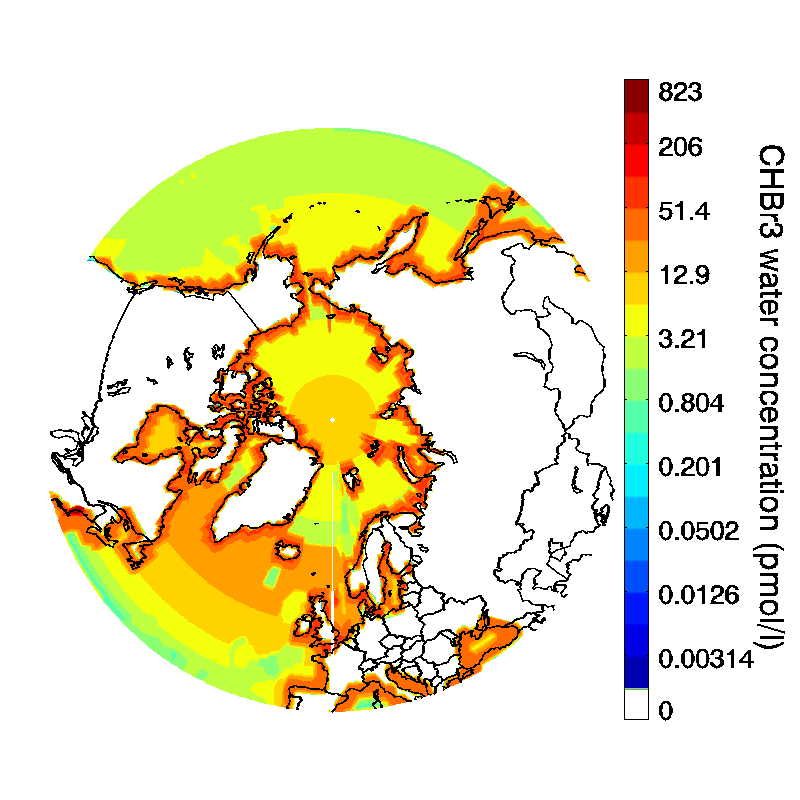
\includegraphics[width=0.5\textwidth]{version_3/CHBr3_waterconcentration.png}
\caption{\chem{CHBr_3} water concentration in \unit{pmol\,l^{-1}} from \citet{ACP:Ziska2013}}
\label{fig:water_con}
\end{figure}
\item[$\bullet$]{\color{blue}P12 L18 and elsewhere in the text: is \emph{ansatz} an accepted English word?}: \emph{Ansatz} is indeed an accepted word in English. See \url{https://en.oxforddictionaries.com/definition/ansatz} for details.
\item[$\bullet$]{\color{blue}P13 Fig.6: Have you thought about including the \chem{CH_2Br_2} and \chem{CHBr_3} photolysis rate vertical profile in a second panel?}
  An early version of the manuscript indeed included a figure of photolysis rate vertical profiles. We have put a figure into the revised manuscript.
  \item[$\bullet$]{\color{blue}P13 L11: ``At about 20\,\unit{hPa}...'' Do you mean a 20\,\unit{hPa} difference from the mean tropopause?}
  Without looking at the corresponding figure, the reference to 20\,\unit{hPa} at this point is indeed not clear. We have rephrased the sentence to clarify that 20\,\unit{hPa} is meant with respect to the mean tropopause: \emph{Within 20\,\unit{hPa} with respect to the mean tropopause, [...]}.
\item[$\bullet$]{\color{blue}Regarding Fig. 9, and considering P8 L1 ``There is an upward shift of the tropopause height of about 8\,\unit{hPa} between present day and future''. Why would you show such a large shift in pressure respect to the mean tropopause ($\pm100$\,\unit{hPa}) if the difference in the tropopause pressure is smaller than 10\,\unit{hPa}? I would expect the changes in the tropopause height to affect only the UTLS, and partitioning between SG and PG, but not the overall total bromine abundances in the middle and upper stratosphere.}
  There are two aspects which we are addressing in Section~\ref{sec:bromine_loading} of our paper. As others have also shown, the future troposphere is warming and enlarging, while the stratosphere is cooling and shrinking. In accordance, the tropopause is rising. We also see an enhancement of vertical tracer transport in tropical regions, pushing younger air further upwards. This air has still a higher amount of SG which have not yet degenerated to PG. This physical effect is in fact shown in Fig.~\ref{fig:annual_mean_change_vsls} and discussed in the beginning of Section~\ref{sec:bromine_loading}. In Figure~\ref{fig:annual_mean_change_relativ_tp}, which is discussed in Section~\ref{subsec:tropopause}, we look at a different aspect. Due to the physical changes, accompanied by a rise of the mean tropopause in the tropics, it is not entirely valid to simply compare VMR at the ``same'' pressure level in the UTLS between present and future. The entire profile is shifted upwards not only the UTLS region, although the UTLS region includes the most extreme example: ``[A]ir which at present is considered stratospheric will be still tropospheric in the future.'' We make this point clearer in the final manuscript version.
\item[$\bullet$]{\color{blue}P15 L14: If the authors are willing to address the impact of VSLS in the future evolution of Antarctic ozone, they should at least compare their results respect to \citet{GRL:Oman2016} and \citet{ACP:Fernandez2017}.}
  We are not in detail addressing changes in the Antarctic ozone hole, but we will include the references and compare our results to these papers.
\item[$\bullet$]{\color{blue}P18 L29: ``... and aerosol formation have been taken into consideration.'' While a full aerosol treatment has been considered for some of the simulations, the sentence gives the impression that an aerosol formation module for VSLS has been considered in this work. I suggest rephrasing to avoid misleading interpretations.}
  Indeed, only a small portion of the entire paper is based on simulations including an aerosol formation treatment (RT1a/RT1b). RT1a/RT1b are only analysed in the context of VSLS influence on future ozone. We do not study aerosols explicitly in this paper and have in fact no special formation mechanism of aerosols involving VSLS. We rewrite the sentence to prevent from misleading interpretations: \emph{While interactive emissions from constant ocean concentrations have been taken into consideration, [...].}
\end{itemize}
\end{itemize}
\newpage

\title{Brominated VSLS and their influence on ozone under a changing climate}

% \Author[affil]{given_name}{surname}
\Author[1]{Stefanie}{Falk}
\Author[1]{Bj\"{o}rn-Martin}{Sinnhuber}
\Author[2]{Gis\`{e}le}{Krysztofiak}
\Author[3]{Patrick}{J\"{o}ckel}
\Author[3]{Phoebe}{Graf}
\Author[4]{Sinikka T.}{Lennartz}

\affil[1]{Institute of Meteorology and Climate Research, Karlsruhe Institute of Technology, Karlsruhe, Germany}
\affil[2]{LPC2E, Universit\'{e} d'Orl\'{e}ans, CNRS, UMR7328, Orl\'{e}ans, France}
\affil[3]{Deutsches Zentrum f\"{u}r Luft- und Raumfahrt e.V., Oberpfaffenhofen, Germany}
\affil[4]{Geomar, Helmholtz-Centre for Ocean Research Kiel, Kiel, Germany}
%% The [] brackets identify the author with the corresponding affiliation. 1, 2, 3, etc. should be inserted.

\runningtitle{Future change in brominated VSLS}

\runningauthor{Falk et al.}

\correspondence{Stefanie Falk (stefanie.falk@kit.edu)}

\received{}
\pubdiscuss{} %% only important for two-stage journals
\revised{}
\accepted{}
\published{}

%% These dates will be inserted by Copernicus Publications during the typesetting process.

\firstpage{1}

\maketitle

\begin{abstract}
Very short-lived \DIFdelbegin \DIFdel{source gases}\DIFdelend \DIFaddbegin \DIFadd{substances}\DIFaddend ~(VSLS) contribute \DIFaddbegin \DIFadd{as source gases }\DIFaddend significantly to the tropospheric and stratospheric bromine loading. At present, an estimated 25\% of stratospheric bromine is of oceanic origin. In this study, we investigate how climate change may impact the ocean--atmosphere flux of brominated VSLS, their atmospheric transport, chemical transformations, and evaluate how these changes will affect stratospheric ozone over the 21st century.\\
Under the assumption of fixed ocean water concentrations and RCP6.0 scenario, we find an increase of the ocean--atmosphere flux of brominated VSLS of about 8--10\% by the end of the 21st century compared to present day.
A decrease in the tropospheric mixing ratios of VSLS and an increase in the lower stratosphere are attributed to changes in atmospheric chemistry and transport. Our model simulations reveal that \DIFdelbegin \DIFdel{, in line with the reduction in the troposphere, }\DIFdelend \DIFaddbegin \DIFadd{this increase is counteracted by a corresponding reduction of inorganic bromine. Therefore }\DIFaddend the total amount of bromine from VSLS in the stratosphere will \DIFdelbegin \DIFdel{decrease during the 21st century}\DIFdelend \DIFaddbegin \DIFadd{not be changed by an increase in upwelling}\DIFaddend . Part of the \DIFdelbegin \DIFdel{apparent }\DIFdelend increase of VSLS in the tropical lower stratosphere results from an increase in the corresponding tropopause height. As the depletion of stratospheric ozone due to bromine depends also on the availability of chlorine, we find the impact of bromine on stratospheric ozone at the end of the 21st century reduced compared to present day.
Thus, these studies highlight the different factors influencing the role of brominated VSLS in a future climate.
\end{abstract}
%
%\clearpage
%
\introduction  %% \introduction[modified heading if necessary]
Ozone is an important trace gas in the Earth's atmosphere. The stratospheric layer of its highest abundance, the ozone layer, absorbs harmful ultraviolet~(UV) radiation threatening all lifeforms on the Earth's surface and acts as a potent greenhouse gas~(GHG). In the troposphere, ozone is considered a harmful pollutant. Catalytic cycles involving bromine and mixed halogen reactions, namely with chlorine, efficiently deplete ozone~\citep[e.g.,][]{ACP:Sinnhuber2009}. The ozone depletion efficiency of bromine is strongly related to the available amount of activated chlorine in the atmosphere~\citep{ACP:Yang2014,GRL:Sinnhuber2015,GRL:Oman2016}. Long-lived, anthropogenically emitted, halogenated source gases~(SG), e.g., \chem{CH_3Br} and Halons, have been restricted by the Montreal protocol and its amendments. Their atmospheric concentrations have started to decline globally~\citep[see][Chap. 1]{WMO2010}. Still, they contribute about 75\% to the overall bromine loading in the stratosphere. The remainder is provided by organic SG of oceanic origin of which methyl bromide (\chem{CH_3Br}), bromoform (\chem{CHBr_3}), and dibromomethane (\chem{CH_2Br_2}) are the most abundant. Minor brominated \DIFdelbegin \DIFdel{VSLS }\DIFdelend \DIFaddbegin \DIFadd{very short-lived substances (VSLS) }\DIFaddend include the mixed bromo-chloro-carbons \chem{CHCl_2Br}, \chem{CHClBr_2}, and \chem{CH_2ClBr}. The tropospheric lifetime of these gases lies between several days to weeks\DIFdelbegin \DIFdel{, hence they are referred to as very short-lived source gases~(VSLS)}\DIFdelend . They are produced by plankton and macroalgae, and are predominantly produced in coastal waters~\citep{JGR:Moore1996,LO:Lin2012,MC:Hughes2013,BGS:Stemmler2015}. Through gas exchange governed by the concentration gradient between ocean water \DIFdelbegin \DIFdel{($c_\text{w}$) and atmosphere($c_\text{w}$)}\DIFdelend \DIFaddbegin \DIFadd{and atmosphere}\DIFaddend , solubility, and wind stress, VSLS are emitted into the atmosphere. Transport to the stratosphere, as shown by different model studies~\citep{ACP:Aschmann2009,GRL:Hossaini2012,ACP:Liang2014}, occurs in tropical regions of deep convection, most importantly the Western Pacific and Maritime Continent, in South East Asia, and over the Gulf of Mexico. Organic SG are transported through the tropical tropopause layer~(TTL) together with their inorganic product gases~(PG). PG are produced through photochemical decomposition of VSLS and provide reactive bromine (\chem{Br_y}, from \chem{Br}, \chem{Br_2}, \chem{HBr}, \chem{BrO}, \chem{BrONO_2}, \chem{BrNO_2}, \chem{BrCl}, and \chem{HOBr}) to the stratosphere. This is schematically shown in Fig.~\ref{fig:vsls_scheme}. In recent years, several approaches have been taken to describe the stratospheric or regional abundance of bromine from VSLS. Top-down scenarios~\citep{JGR:Warwick2006, ACP:Liang2010, ACP:Ordonez2012} match atmospheric observations by setting constant fluxes or boundary concentrations. Bottom-up scenarios~\citep[e.g.,][]{ACP:Ziska2013} developed emission climatologies by extrapolating measurements in the surface ocean and marine boundary layer and calculate emissions accordingly. As shown by \citet{ACP:Lennartz2015}, the bottom-up fluxes based on the oceanic water concentrations of \citet{ACP:Ziska2013} are in good agreement with available atmospheric VSLS observations. \DIFaddbegin \DIFadd{Recently, \mbox{%DIFAUXCMD
\citet{JAC:Ziska2017} }%DIFAUXCMD
have investigated the future evolution of the ocean--atmosphere fluxes of VSLS through the 21st century based on Coupled Model Intercomparison Project~(CMIP)~5 model output and fixed atmospheric VSLS concentrations. They found fluxes of }\chem{CH_2Br_2} \DIFadd{and }\chem{CHBr_3} \DIFadd{increasing by 6.4\% (23.3\%) and 9.0\% (29.4\%), respectively, dependent on the Representative Concentration Pathways~(RCP)~2.6 (RCP8.0) scenario.}\DIFaddend \\
In this study, we will address the open questions on how these oceanic emissions of VSLS evolve in response to a changing climate \DIFaddbegin \DIFadd{and changing atmospheric concentrations }\DIFaddend (Section~\ref{sec:emission_trends}), how transport and \DIFaddbegin \DIFadd{tropospheric }\DIFaddend chemistry influence the stratospheric bromine abundance in a changing climate (Section~\ref{sec:bromine_loading}), and how \DIFaddbegin \DIFadd{stratospheric }\DIFaddend ozone will be affected by the assumed changes in VSLS abundance (Section~\ref{sec:ozone_depletion}). Details about the model and simulations used in this study will be given in Section~\ref{sec:model_exp}.
%
\begin{figure}[t]
  \centering
  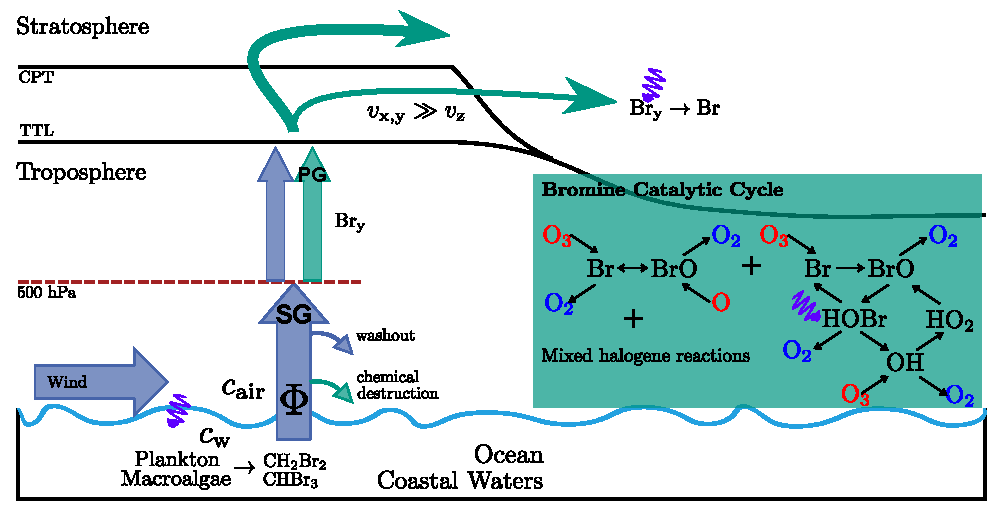
\includegraphics[width=8.3cm]{fig01}
  \caption{Scheme of VSLS emission and catalytic cycle of ozone depletion involving bromine. (left) VSLS are produced by plankton and macroalgae predominantly in coastal waters. They are emitted through gas exchange between ocean ocean and atmosphere. These organic source gases (SG) undergo chemical transformation into inorganic product gases (PG). Both are convectively transported through the tropical tropopause layer (TTL). Through photochemical decomposition, reactive bromine \chem{Br_y} is provided to the stratosphere. (right) Two examples of catalytic cycles of ozone depletion involving bromine. A $+$ indicates increasing order of catalytic complexity. Reactants are shown in red, catalysts in black, and products in blue. Photochemical reactions are indicated by a violet wave.}
  \label{fig:vsls_scheme}
\end{figure}
%
\section{Model and experiments}
\label{sec:model_exp}
All model experiments have been performed using the ECHAM/MESSy Atmospheric Chemistry~(EMAC) model~\citep{GMD:Joeckel2010}. Table~\ref{tab:experiments} gives an overview over the key-factors of the simulations.\\
Future changes in fluxes of brominated VSLS from the ocean are studied with a free-running long-term simulation (SC\_free, 1979--2100) using a simplified chemistry (Section~\ref{sec:emission_trends}), augmented by a similar simulation, but nudged towards the European Centre for Medium-Range Weather Forecasts~(ECMWF) Re-Analysis (ERA)--Interim over the period 1979--2012. Therein, \DIFaddbegin \DIFadd{VSLS }\DIFaddend emission fluxes are computed online from prescribed sea water concentrations. The \DIFdelbegin \DIFdel{simplified-chemistry }\DIFdelend \DIFaddbegin \DIFadd{simplified chemistry }\DIFaddend simulations use EMAC version 2.50 with submodels \texttt{airsea} \citep{ACP:Pozzer2006} (\DIFdelbegin \DIFdel{$k_\mathrm{w}$ parametrization ~\mbox{%DIFAUXCMD
\citet{GRS:Nightingale2000}}%DIFAUXCMD
}\DIFdelend \DIFaddbegin \DIFadd{with $k_\mathrm{w}=0.222\,u^2+0.333\,u$ parametrization quadratic with respect to wind speed~\mbox{%DIFAUXCMD
\citep{GRS:Nightingale2000}}%DIFAUXCMD
}\DIFaddend ), \texttt{cloud}, \texttt{cloudopt}, \texttt{convect} (with operational ECMWF convection scheme), \texttt{cvtrans}, \texttt{ddep} \citep{ACP:Kerkweg2006b}, \texttt{\DIFdelbegin \DIFdel{ptracs}\DIFdelend \DIFaddbegin \DIFadd{ptrac}\DIFaddend } \citep{ACP:Joeckel2008}, \texttt{rad}, \texttt{scav} \citep{ACP:Tost2006}, \texttt{surface}, and \texttt{tnudge} \citep{ACP:Kerkweg2006}\DIFdelbegin \DIFdel{(}\DIFdelend \DIFaddbegin \DIFadd{. The }\DIFaddend set-up \DIFaddbegin \DIFadd{is }\DIFaddend as in~\citet{ACP:Lennartz2015,ACP:Hossaini2016}\DIFdelbegin \DIFdel{). The tracer }\DIFdelend \DIFaddbegin \DIFadd{. Chemical reactions are not computed interactively, e.g.,  via the EMAC submodul }\texttt{\DIFadd{mecca}}\DIFadd{~\mbox{%DIFAUXCMD
\citep{GMD:Sander2011}}%DIFAUXCMD
. The VSLS }\DIFaddend lifetime due to reaction with \chem{OH} has been fixed to monthly mean values from \DIFaddbegin \DIFadd{the }\DIFaddend National Centre for Meteorological Research~(CNRM)~\citep{GMD:Michou2011,GMD:Morgenstern2016} model calculations, while photolysis rates are computed within the EMAC submodel \texttt{jval}~\citep{GMD:Sander2014}. \DIFdelbegin \DIFdel{In these simulations }\DIFdelend \DIFaddbegin \DIFadd{Only in these simulations with simplified chemistry}\DIFaddend , \chem{OH} concentrations have been set to zero in the lower troposphere (700--1000\,\unit{hPa}) to reduce the variability of ground level volume mixing ratio~(VMR) of VSLS. \DIFaddbegin \DIFadd{The chemical lifetime of VSLS in the lower troposphere is therefore overestimated. Due to the longer lifetime, VSLS are more abundant in the lower troposphere leading to a flux suppression. }\DIFaddend Water concentrations of \chem{CH_2Br_2} and \chem{CHBr_3} have been held constant using the climatology of~\citet{ACP:Ziska2013}. For mixed bromo-chloro-carbons (\chem{CHBrCl_2}, \chem{CHBr_2Cl}, \chem{CH_2BrCl}), water concentrations have been estimated by scaling \chem{CHBr_3} concentrations to obtain a better agreement between model simulation and tropical mean profile and surface observations of these VSLS. \DIFdelbegin \DIFdel{Bromine produced by VSLS decomposition is commuted into }\DIFdelend \DIFaddbegin \DIFadd{Based on the lifetime estimate, VSLS are decomposed and converted to }\DIFaddend \chem{Br_y}. The \DIFdelbegin \DIFdel{distribution }\DIFdelend \DIFaddbegin \DIFadd{partitioning of }\chem{Br_y} \DIFaddend into \chem{Br}, \DIFaddbegin \chem{Br_2}\DIFadd{, }\DIFaddend \chem{HBr}, \chem{BrO}, \chem{BrONO_2}, \chem{BrNO_2}, \chem{BrCl}, \DIFaddbegin \DIFadd{and }\DIFaddend \chem{HOBr} in these simplified chemistry simulations has been computed offline from a full-chemistry EMAC simulation of one year duration with six hourly output. Scavenging is applied to \chem{Br}, \chem{Br_2}, \chem{HBr}, \chem{BrNO_2}, \chem{BrONO_2}, \chem{BrCl}, and \chem{HOBr}. Concentrations of \chem{CO_2}, \chem{CH_4}, \chem{CFC}, and \chem{N_2O} in SC\_free are taken from a CNRM CM5 model~\citep{CD:Voldoire2013} simulation with \DIFdelbegin \DIFdel{Representative Concentration Pathways~(RCP)~6.0 }\DIFdelend \DIFaddbegin \DIFadd{RCP6.0 }\DIFaddend scenario~\citep{EJ:Fujino2006,GEE:Hijioka2008}.\\
%
Data of a full-chemistry long-term simulation~\citep[RC2-base-05,][]{GMD:Joeckel2016} over a time span of 150 years (1950--2100) and performed as part of a Chemistry-Climate Model Initiative~(CCMI) recommended set of simulations by the Earth System Chemistry-Climate Modelling~(ESCiMo) consortium will be used for studying changes in transport and \DIFdelbegin \DIFdel{partitioning }\DIFdelend \DIFaddbegin \DIFadd{photochemical transformation }\DIFaddend of bromine species (Section~\ref{sec:bromine_loading}). In this simulation, VSLS fluxes have been held constant following scenario five of~\citet{JGR:Warwick2006}.\\
An intermediate-term experiment, consisting of a set of two simulations and spanning the years 2075--2100, has been performed for assessing implications on ozone depletion in a future climate with significantly lower chlorine loading in the atmosphere (Section~\ref{sec:ozone_depletion}). The simulations named RT1a and RT1b both include online computation of aerosol formation. Fluxes of \chem{CH_2Br_2} and \chem{CHBr_3} are computed online from sea water concentrations of \DIFdelbegin \DIFdel{~}\DIFdelend \citet{ACP:Ziska2013} using the EMAC submodel \texttt{airsea} \DIFdelbegin \DIFdel{(with the \mbox{%DIFAUXCMD
\citet{JGRC:Wanninkhof1992} }%DIFAUXCMD
}\DIFdelend \DIFaddbegin \DIFadd{as in RC2-base-05 with the }\DIFaddend $k_\mathrm{w}$ parametrization \DIFdelbegin \DIFdel{as in RC2-base-05)in case of RT1a}\DIFdelend \DIFaddbegin \DIFadd{according to \mbox{%DIFAUXCMD
\citet{JGRC:Wanninkhof1992}}%DIFAUXCMD
, which is strictly quadratic with respect to wind speed ($k_\mathrm{w}=0.31\,u^2$)}\DIFaddend . For assessing the impact of VSLS on ozone, all VSLS emissions have been switched off in RT1b. \DIFdelbegin %DIFDELCMD < \\
%DIFDELCMD < %%%
\DIFdelend \DIFaddbegin \DIFadd{The impact of various $k_\mathrm{w}$ parametrizations on VSLS emission has been previously studied. The differences on the global level are <15\% (cf. Tab.~4 in \mbox{%DIFAUXCMD
\citet{ACP:Lennartz2015} }%DIFAUXCMD
when comparing \mbox{%DIFAUXCMD
\citet{GRS:Nightingale2000} }%DIFAUXCMD
and \mbox{%DIFAUXCMD
\citet{GRL:Wanninkhof1999}}%DIFAUXCMD
). For wind speeds exceeding 10\,}\unit{ms^{-1}} \DIFadd{the \mbox{%DIFAUXCMD
\citet{JGRC:Wanninkhof1992} }%DIFAUXCMD
$k_\mathrm{w}$ parametrization diverges slightly stronger towards higher transfer velocities compared to the \mbox{%DIFAUXCMD
\citet{GRS:Nightingale2000} }%DIFAUXCMD
parametrization (cf. Fig.~1 in \mbox{%DIFAUXCMD
\citet{GRL:Wanninkhof1999} }%DIFAUXCMD
and Fig.~2 in \mbox{%DIFAUXCMD
\citet{ACP:Lennartz2015}}%DIFAUXCMD
). Regarding integrated global emissions of VSLS, both parametrizations result in similar fluxes, given that the mean global wind speed lies in a range where these parameterizations do not differ drastically. However, the \mbox{%DIFAUXCMD
\citet{GRS:Nightingale2000} }%DIFAUXCMD
parameterization reacts more sensitive to changes in wind speed, which introduces a further uncertainty when assessing changes over time in a changing climate.
}\DIFaddend The full-chemistry experiments use EMAC version 2.51 (RC2-base-05) and 2.52 (RT1a/b), respectively. The dynamics have not been specified except for a weak nudging of the equatorial wind quasi-biennial oscillation~(QBO). RC2-base-05 combines hindcast with future projections. The set-up of RT1a and RT1b is almost identical to RC2-base-05, thus we refer to the corresponding paper by the ESCiMo consortium~\citep{GMD:Joeckel2016} for general information. The major difference lies in the aforementioned treatment of VSLS emission, which is handled analogous to SC\_free, except for mixed bromo-chloro-carbons emissions taken from~\citet{JGR:Warwick2006}. Since heterogeneous reaction and chlorine activation are important for the depletion process of ozone, \DIFaddbegin \DIFadd{tropospheric and stratospheric }\DIFaddend aerosol formation is computed online using the submodel \texttt{GMXe}~\citep{GMD:Pringle2010} of EMAC. The set-up has been adapted from RC1-aero-07~\citep{GMD:Joeckel2016} with modifications as \DIFdelbegin \DIFdel{in}\DIFdelend \DIFaddbegin \DIFadd{described by}\DIFaddend ~\citet{ACP:Bruehl2012,JGR:Bruehl2015}. Radiation coupling had been activated in \texttt{GMXe}, but cloud coupling had not been activated. In this regard, an additional oceanic sulfur source, carbonyl sulfide (COS), which is a major source of stratospheric sulfur has been included in addition to dimethyl sulfide (DMS). Whereas the emission of the latter is computed from prescribed ocean concentrations, constant fluxes of COS have been adopted from~\citet{JGR:Kettle2002}. Additional reaction pathways of sulfur have been enabled accordingly. RT1a and RT1b have been initialized with available monthly mean values from RC2-base-05. COS has been initialized from a simulation which results have been published recently~\citep{GRL:Glatthor2015}, including an artificially increased oceanic source to close the atmospheric budget.\\
The model's spatial resolution is T42L39MA for the simplified chemistry experiments, T42L47MA for RC2-base-05\DIFdelbegin \DIFdel{respectively }\DIFdelend \DIFaddbegin \DIFadd{, and }\DIFaddend T42L90MA for RT1a/RT1b, \DIFaddbegin \DIFadd{respectively, }\DIFaddend corresponding to a $2.8^\circ\times 2.8^\circ$ grid, with a top level at 0.01\,\unit{hPa}\DIFaddbegin \DIFadd{, and 39, 47, or 90 vertical hybrid-pressure levels. The mean tropical troposphere (below 100\,}\unit{hPa}\DIFadd{) is discretised into 16, 26, or 27 levels, and the mean tropical stratosphere between 100\,}\unit{hPa} \DIFadd{and 1\,}\unit{hPa} \DIFadd{consists of 15, 15, or 48 levels, respectively}\DIFaddend . Emissions of GHG follow the RCP6.0 scenario and sea surface temperature~(SST) and sea ice cover~(SIC) are prescribed from Hadley Centre Global Environment Model version 2~(HadGEM2) forced with the RCP6.0 scenario for all simulations accordingly.
%
\begin{table*}[t]
  \centering
  \caption[]{EMAC model experiments used in this study. All experiments follow the RCP6.0 scenario of GHG emissions and have accordingly prescribed SST and SIC from HadGEM2.}
  \begin{tabular}{lcccccc}
    \tophline
    Experiment & Model Version & Resolution & Time-Span & Chemistry & VSLS Emission & Interactive Aerosols\\
    \middlehline
    SC\_nudged & 2.50 & T42L39MA & 1979--2012 & simplified bromine & \texttt{airsea} & no\\
    SC\_free & 2.50 & T42L39MA & 1979--2100 & simplified bromine & \texttt{airsea} & no\\
    RC2-base-05 & 2.51 & T42L47MA & 1950--2100 & full & \citet{JGR:Warwick2006} & no\\
    RT1a & 2.52 & T42L90MA & 2075--2100 & full + sulfur & \texttt{airsea} & yes\\
    RT1b & 2.52 & T42L90MA & 2075--2100 & full + sulfur & none & yes\\
    \bottomhline
  \end{tabular}
  \label{tab:experiments}
\end{table*}
\section{Long-term Trends in Oceanic Emission Fluxes}
\label{sec:emission_trends}
In this section, we investigate how a changing climate may influence emission fluxes of VSLS from the ocean. We will assess the impact of changing physical factors (e.g., SST, SIC, and wind speed) on ocean--atmosphere gas exchange driven by the RCP6.0 scenario. Here we assume constant oceanic concentrations of VSLS over the course of the century (following~\citet{ACP:Ziska2013,ACP:Lennartz2015}). This specific assumption might not hold since the effects of climate change, e.g., increase of ocean temperature, acidification, change of salinity, and nutrient input, on marine organisms and thus the production of \chem{CH_2Br_2} and \chem{CHBr_3} is not yet fully understood. Recent combined marine ecosystem model studies imply a global decrease of net primary production~(NPP) by plankton over the course of the 21st century~\citep{BGS:Laufkoetter2015,BGS:Laufkoetter2016}. However, the impact on bromocarbon concentration, predominantly produced by macroalgae in coastal regions, remains unclear.\\
%
As implemented in the EMAC submodel \texttt{airsea}~\citep{ACP:Pozzer2006}, the flux of a gas dissolved in ocean water to the atmosphere is governed by its concentration gradient $\Delta c$ and transfer velocity $k$, 
\begin{align}
  \label{eq:airsea}
  \Phi &= k\cdot \Delta c \\ \notag
       &= k\cdot \left(c_\text{w} - H\cdot c_\text{air}\right),
\end{align}
with $k = \left(1/k_\mathrm{w}+R\cdot H \cdot T_\mathrm{air}/k_\mathrm{air}\right)^{-1}$, wherein, $R$ is the universal gas constant and $H$ is the Henry coefficient for a specific gas. The transfer velocity depends largely on \DIFdelbegin \DIFdel{temperature $T$ }\DIFdelend \DIFaddbegin \DIFadd{air temperature $T_\text{air}$ }\DIFaddend and surface wind speed\DIFaddbegin \DIFadd{, which is taken into account by distinguishing between water- and air-side transport velocities ($k_\text{w}$, $k_\text{air}$). $k_\mathrm{w}$ is a polynomial function of wind speed depending on the chosen parametrization as mentioned in Section~\ref{sec:model_exp}}\DIFaddend . The corresponding water and atmospheric concentrations are named $c_\mathrm{w}$ and $c_\mathrm{air}$.\\ 
In Fig.~\ref{fig:timeseries_integrated_seasonal_flux}, the difference of VSLS fluxes with respect to the start of the simulation in 1979 is shown for the free-running and nudged \DIFdelbegin \DIFdel{simplified-chemistry }\DIFdelend \DIFaddbegin \DIFadd{simplified chemistry }\DIFaddend simulation. For both, \chem{CH_2Br_2} and \chem{CHBr_3}, all zonal bands display linearly rising fluxes. The strongest increase with respect to 1979 values is found in the tropical zone (20$^\circ$~N--20$^\circ$~S) with roughly 2.5\,\unit{\mathrm{Gg\,yr^{-1}}} and 13\,\unit{\mathrm{Gg\,yr^{-1}}} for \chem{CHBr_3} and \chem{CH_2Br_2} respectively. Relative to the absolute \DIFdelbegin \DIFdel{zonal }\DIFdelend \DIFaddbegin \DIFadd{value of the zonally averaged }\DIFaddend fluxes, this yields an increase of about 10\% over the course of the century (Table~\ref{tab:relative_flux_increase}). The increase is slightly stronger in the southern tropics. The strongest relative increase in flux is found in the northern hemisphere polar region (90$^\circ$~N--50$^\circ$~N), with 25\% and roughly 55\% for \chem{CHBr_3} and \chem{CH_2Br_2}, respectively.\\
%
\begin{table*}[t]
  \centering
  \caption[]{Average absolute flux \DIFdelbeginFL \DIFdelFL{in }\DIFdelendFL \DIFaddbeginFL \DIFaddFL{for the year }\DIFaddendFL 2000 in \unit{\mathrm{Gg\,yr^{-1}}} and percentage of relative increase in VSLS flux between 2000 and 2100 from SC\_free. The numbers have been obtained by linear regression of the data shown in Fig.~\ref{fig:timeseries_integrated_seasonal_flux} and evaluated at the given years.}
  \begin{tabular}{r@{--}l  r@{.}l r@{.}l r@{.}l r@{.}l}
    \tophline
     \multicolumn{2}{c}{Region} & 
     \multicolumn{4}{c}{\chem{CH_2Br_2}} & 
     \multicolumn{4}{c}{\chem{CHBr_3}}\\
     \multicolumn{2}{c}{} &
     \multicolumn{2}{l}{(\unit{\mathrm{Gg\,yr^{-1}}})} &  \multicolumn{2}{l}{(\%)} &
     \multicolumn{2}{l}{(\unit{\mathrm{Gg\,yr^{-1}}})} &  \multicolumn{2}{l}{(\%)}\\
     \middlehline
     $\mathrm{90^\circ N}$ & $\mathrm{50^\circ N}$ & 0&6 & 54&6 & 23&5  & 25&0\\
     $\mathrm{50^\circ N}$ & $\mathrm{20^\circ N}$ & 8&2 & 14&6 & 41&7  & 8&7\\
     $\mathrm{20^\circ N}$ & $\mathrm{0}$ & 19&2 & 6&6 & 52&4  & 8&6\\
     $\mathrm{0}$ & $\mathrm{20^\circ S}$ & 5&5 & 11&9 & 44&4  & 10&0\\
     $\mathrm{20^\circ S}$ & $\mathrm{50^\circ S}$ & 4&3 & 18&0 & 33&2  & 8&2\\
     $\mathrm{50^\circ S}$ & $\mathrm{90^\circ S}$ & 6&9 & 6&8 & 12&7  & 8&9\\
     \bottomhline
  \end{tabular}
  \label{tab:relative_flux_increase} 
\end{table*}
%
Regarding the changing physical factors, the HadGEM2 prescribed SSTs are increasing almost linearly over the course of the century (Fig.~\ref{fig:hadgem2_input}a). Under the RCP6.0 scenario, this increase in SST ranges between 1\,\unit{^\circ\,C}--3.5\,\unit{^\circ\,C}. The weak rise in Antarctic SST is accompanied by a weakly increasing Antarctic flux of VSLS. The corresponding HadGEM2 prognosticated retreat of Arctic sea ice is shown in Fig.~\ref{fig:hadgem2_input}b. Sea ice is not regarded as a source of VSLS in our study and therefore only acts as a lid blocking the ocean to atmosphere flux. \DIFaddbegin \DIFadd{Since the water concentrations from \mbox{%DIFAUXCMD
\citet{ACP:Ziska2013} }%DIFAUXCMD
used in our simulations do not take SIC into account, water concentrations have been extrapolated for regions typically covered by ice at present. In the }\texttt{\DIFadd{airsea}} \DIFadd{submodel, if SIC (fraction of grid box) is larger than 0.5, the transfer velocity ($k_\mathrm{w}$) is equal to zero, in other cases $k_\mathrm{w}$ is scaled depending on the fraction of SIC. }\DIFaddend Hence, a polar sea which is to a large extent free of sea ice \DIFdelbegin \DIFdel{will have }\DIFdelend \DIFaddbegin \DIFadd{has }\DIFaddend increased fluxes of VSLS \DIFaddbegin \DIFadd{in our future simulations. However, there are large uncertainties regarding the VSLS water concentrations in the future polar sea, for the polar ecosystem as a whole is undergoing a drastic change}\DIFaddend . In accordance \DIFaddbegin \DIFadd{to the general increase in flux}\DIFaddend , the Arctic August--September maximum of flux is expected to be more pronounced. 
%DIF < Zonally averaged seasonal cycles of fluxes are shown in Fig.~\ref{fig:integrated_seasonal_flux} for both VSLS species. Solid lines herein refer to a present day average (1990--2000) and dashed lines to future (2090--2100). 
\DIFdelbegin \DIFdel{Distinct maxima in the seasonal cycles are found for summer months on both hemispheres and minima occurring }\DIFdelend %DIF >  
\DIFaddbegin \DIFadd{On both hemispheres, seasonal cycles in zonally averaged VSLS fluxes peak in the summer months and show minima }\DIFaddend in late winter. There is a slightly stronger increase of fluxes in the future during the time periods of maxima, but no change in phase. \DIFdelbegin \DIFdel{In case of }\DIFdelend \DIFaddbegin \DIFadd{Negative emissions representing a net sink of atmospheric }\DIFaddend \chem{CH_2Br_2} \DIFdelbegin \DIFdel{, even negative emissions }\DIFdelend are found during winter at high-latitudes on the northern hemisphere. In the northern tropics, \chem{CHBr_3} shows a distinct maximum in northern hemisphere summer, while the southern tropics do not display any seasonal cycle. Albeit increased ocean--atmosphere fluxes in the future, only taking the changes of physical factors into account, seasonal cycles remain largely the same. In our simulations, zonally averaged absolute wind speed at 10\,\unit{m} is only slightly changing over the course of the 21st century \DIFaddbegin \DIFadd{and with varying sign }\DIFaddend (-4--2\%). Thus, it is indicated by our simulations \DIFaddbegin \DIFadd{but not explicitly shown}\DIFaddend , that the important factor regarding an increase of ocean--atmosphere flux of VSLS is the change in SSTs.\\
%
In Fig.~\ref{fig:gisele-vsls-profiles}, resulting VMR profiles of organic (\chem{Br_{org}}) and inorganic bromine (\chem{Br_y}) from VSLS are shown. VSLS data have been averaged over a time period 1990--2000 and 2090--2100. The VMR profile of \chem{Br_{org}} displays a steep decline in the lower troposphere (400--1000\,\unit{hPa}) by more than 50\% of ground level VMR, stays almost constant before entering the stratosphere, where VSLS are quickly dissociated. Comparing present day and future values (keeping in mind that \chem{OH} \DIFdelbegin \DIFdel{concentration }\DIFdelend \DIFaddbegin \DIFadd{concentrations }\DIFaddend are nudged towards monthly mean values of \chem{OH} and photolysis rates are fixed in SC\_free), \chem{Br_{org}} is found to have increased \DIFdelbegin \DIFdel{through out }\DIFdelend \DIFaddbegin \DIFadd{throughout }\DIFaddend the atmosphere by about 0.1--0.4\,\unit{ppt}. \DIFdelbegin \DIFdel{In }\DIFdelend \DIFaddbegin \DIFadd{Surface values of VSLS increase by 0.47\,}\unit{ppt} \DIFadd{(9\%), while in }\DIFaddend the lower stratosphere, \DIFdelbegin \DIFdel{this }\DIFdelend \DIFaddbegin \DIFadd{the }\DIFaddend increase amounts to \DIFdelbegin \DIFdel{about }\DIFdelend 0.3\,\unit{ppt} (8\%). VMR of \chem{Br_y} is increased from the lower stratosphere upwards by roughly 0.4\,\unit{ppt} (10\%). These changes in the vertical profiles can be attributed to enhanced emissions in a future climate which, as shown, are of the order of 10\% \DIFaddbegin \DIFadd{in the tropics}\DIFaddend .\\
%
As can be inferred from Eq.~(\ref{eq:airsea}), ocean--atmosphere fluxes are sensitive to the abundance of VSLS in the atmosphere as well as a differing wind speed parametrization. An increased chemical dissociation of VSLS in the lowermost troposphere (e.g., due to a probable future increase in \chem{OH}) would reduce the atmospheric concentration and therefore increase the flux from the ocean to the atmosphere without \DIFaddbegin \DIFadd{necessarily }\DIFaddend increasing the actual amount \DIFaddbegin \DIFadd{of bromine }\DIFaddend which is transported to the stratosphere. \DIFaddbegin \DIFadd{The total amount of bromine from VSLS transported through the UTLS strongly depends on the washout of inorganic PG (}\chem{Br_y^{VSLS}}\DIFadd{) and hence on the partitioning and heterogeneous reactions converting }\chem{Br_y^{VSLS}} \DIFadd{between soluble, e.g., }\chem{HBr}\DIFadd{, }\chem{HOBr}\DIFadd{, and insoluble, e.g., }\chem{BrO}\DIFadd{, species~\mbox{%DIFAUXCMD
\citep[e.g.][]{ACP:Aschmann2009,ACP:Liang2014}}%DIFAUXCMD
. Since }\chem{OH} \DIFadd{concentrations in the lower troposphere have been set to zero in SC\_free, the atmospheric lifetime and the resulting abundance of VSLS in the lower troposphere is enhanced. Therefore, the total ocean--atmosphere flux is suppressed. }\DIFaddend In this regard, fluxes from RT1a \DIFaddbegin \DIFadd{at the end of the 21st century }\DIFaddend have been compared to SC\_free \DIFdelbegin \DIFdel{in 2100. }\DIFdelend \DIFaddbegin \DIFadd{within the same time period. }\DIFaddend Much stronger fluxes (1.3--1.5 times) have been found in \DIFdelbegin \DIFdel{the former simulation }\DIFdelend \DIFaddbegin \DIFadd{RT1a in comparison to SC\_free. Particularly, no net sink for }\chem{CH_2Br_2} \DIFadd{occurs at high latitudes in RT1a. This partly explains the smaller increase }\DIFaddend in comparison to \DIFdelbegin \DIFdel{the latter}\DIFdelend \DIFaddbegin \DIFadd{results recently published by~\mbox{%DIFAUXCMD
\citet{JAC:Ziska2017}}%DIFAUXCMD
. \mbox{%DIFAUXCMD
\citet{JAC:Ziska2017} }%DIFAUXCMD
diagnosed the flux from parameters such as SST and wind speed for a fixed VSLS concentration gradient and for different CMIP5 model simulations. They found an increase in flux of }\chem{CHBr_3}\DIFadd{/}\chem{CH_2Br_2} \DIFadd{of 29.4\%/23.3\% for the RCP8.0 scenario and 9.0\%/6.4\% for RCP2.6, respectively. In addition to the smaller absolute fluxes due to the artificial suppression caused by setting }\chem{OH} \DIFadd{to zero in the lower troposphere, we expect a smaller increase in flux from a theoretical point, taking Eq.~\ref{eq:airsea} in to account, since we allow atmospheric concentrations to respond to changing flux}\DIFaddend . Underlying changes in photochemical dissociation and tracer transport due to a changing climate have not been disentangled at this point and will be studied in detail in the following section.
%
\begin{figure}[t]
  \centering
  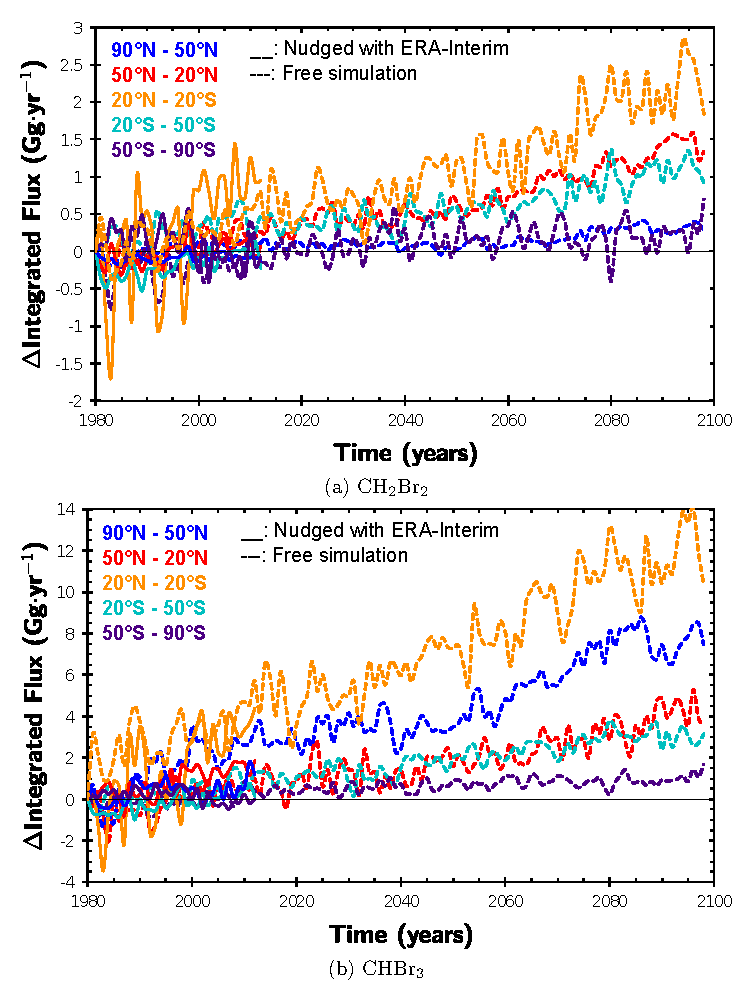
\includegraphics[width=8.3cm]{fig02}
  \caption[]{Difference of integrated flux separated in different zonal bands. Simplified chemistry EMAC simulation (SC\_free and SC\_nudged) with \texttt{airsea} gas exchange, water concentrations held constant. Solid lines represent ERA--Interim nudged (1979--2012) and dashed lines free-running (1979--2100).}
  \label{fig:timeseries_integrated_seasonal_flux}
\end{figure}
%
\begin{figure}[t]
  \centering
  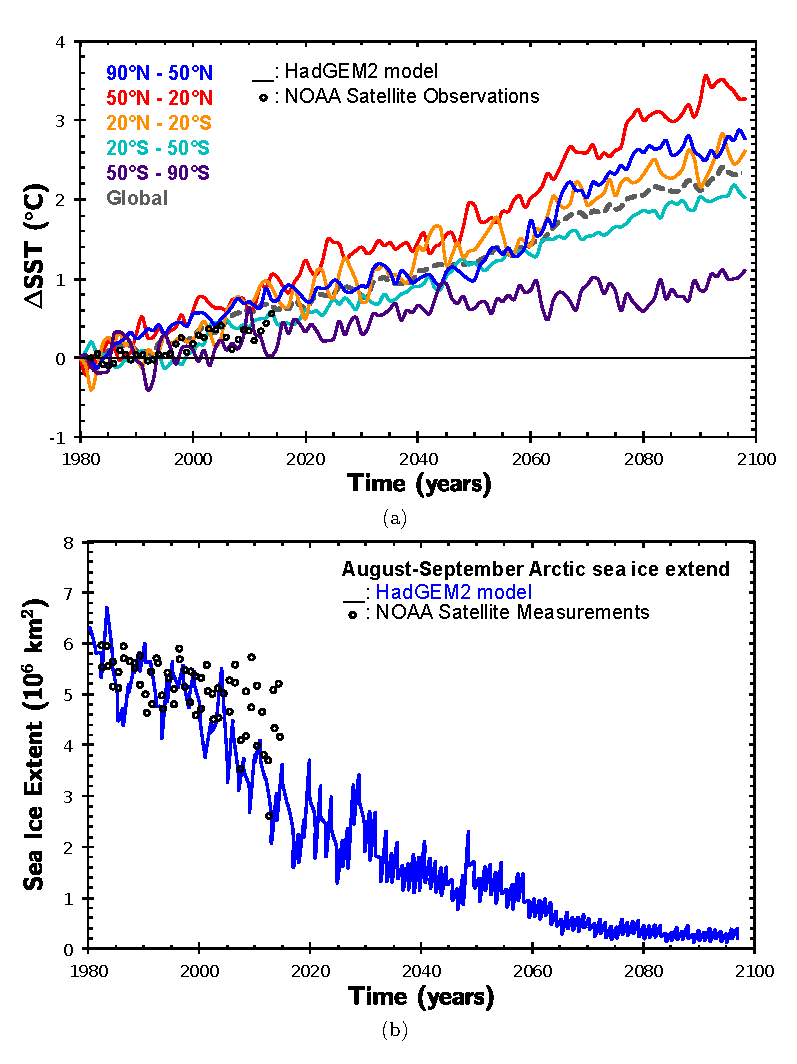
\includegraphics[width=8.3cm]{fig03}
  \caption[]{HadGEM2 prescribed ocean properties in the \DIFdelbeginFL \DIFdelFL{simplified-chemistry }\DIFdelendFL \DIFaddbeginFL \DIFaddFL{simplified chemistry }\DIFaddendFL simulations compared to National Oceanic and NOAA Optimum Interpolation~(OI)~V2 fields~\citep{JC:Reynolds2002}. (a) Change in sea surface temperature for different latitude bands. Global average is shown as dashed gray line. (b) Arctic sea ice extend in August and September.}
  \label{fig:hadgem2_input}
\end{figure}
%
%DIF < \begin{figure}[t]
%DIF <   \centering
%DIF <   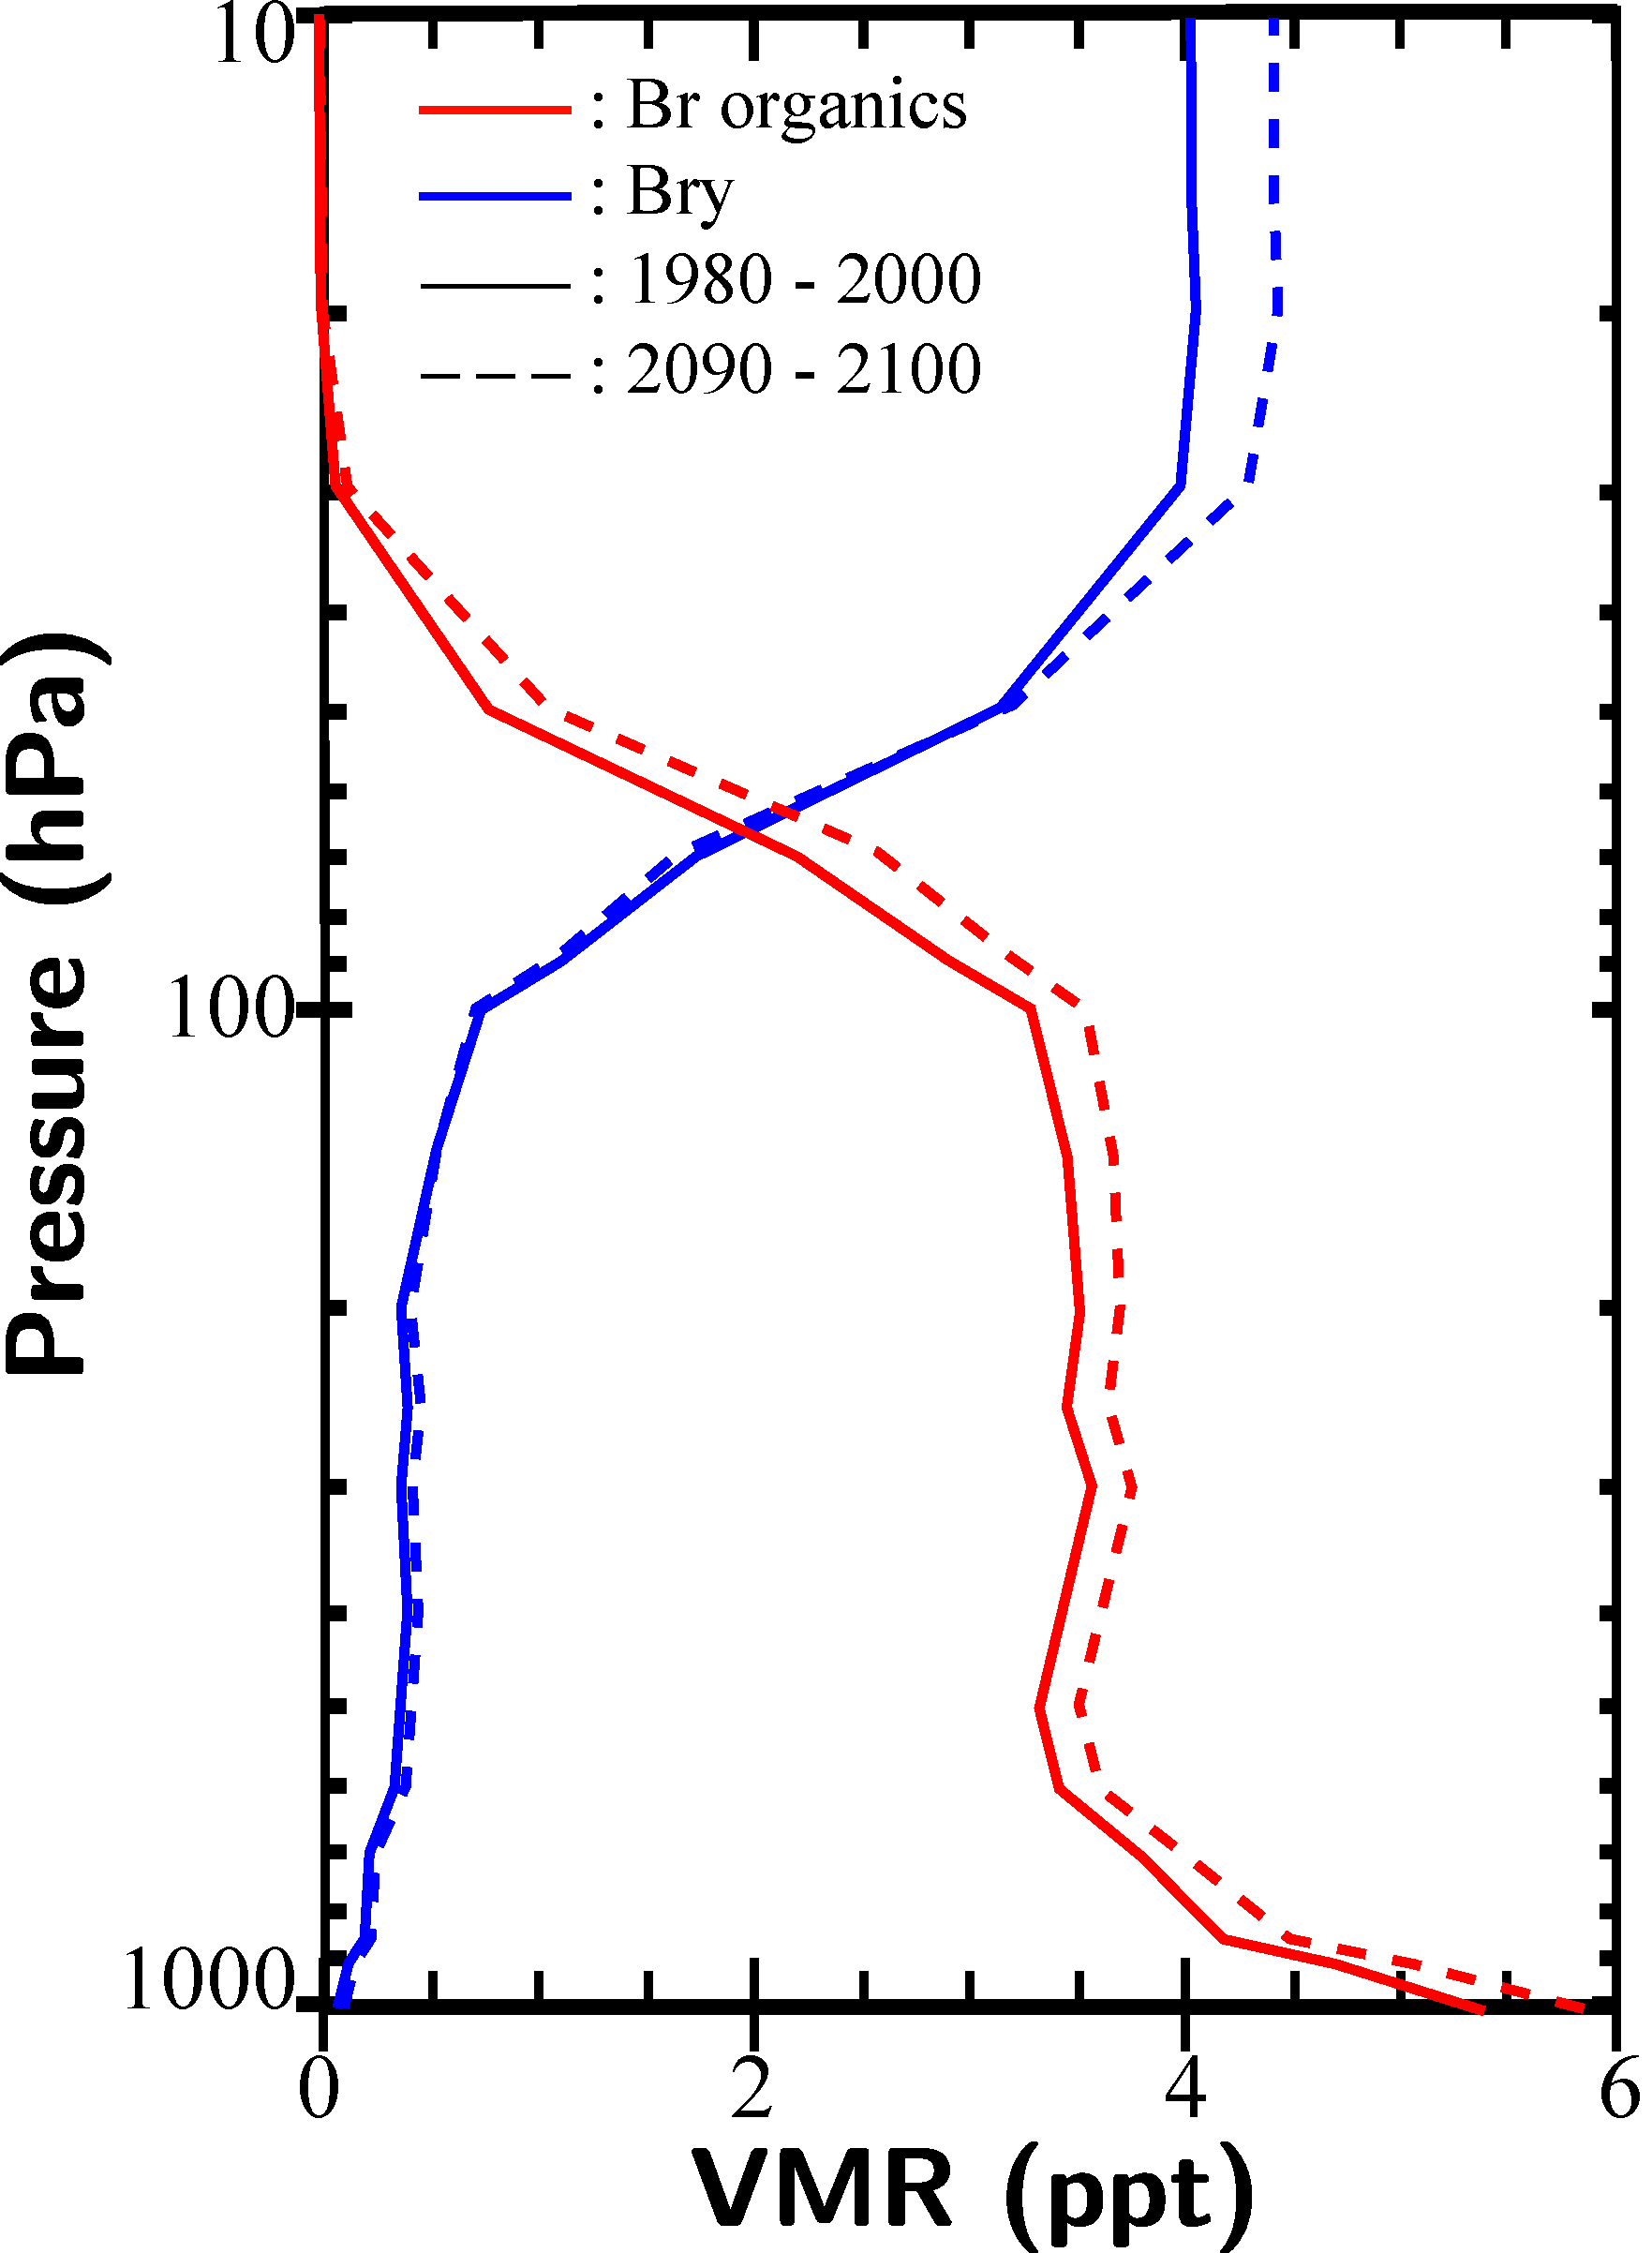
\includegraphics[width=8.3cm]{fig04}
%DIF <   \caption[]{Seasonal variation of integrated VSLS fluxes from EMAC simplified-chemistry simulation (1979--2100). 10 year averaged zonal means are shown with standard error on mean as shaded error bands. Solid lines refer to present-day mean (1990--2000) and dashed lines to future mean (2090--2100)}
%DIF <   \label{fig:integrated_seasonal_flux}
%DIF < \end{figure}
%DIF < 
\begin{figure}[t]
  \centering
  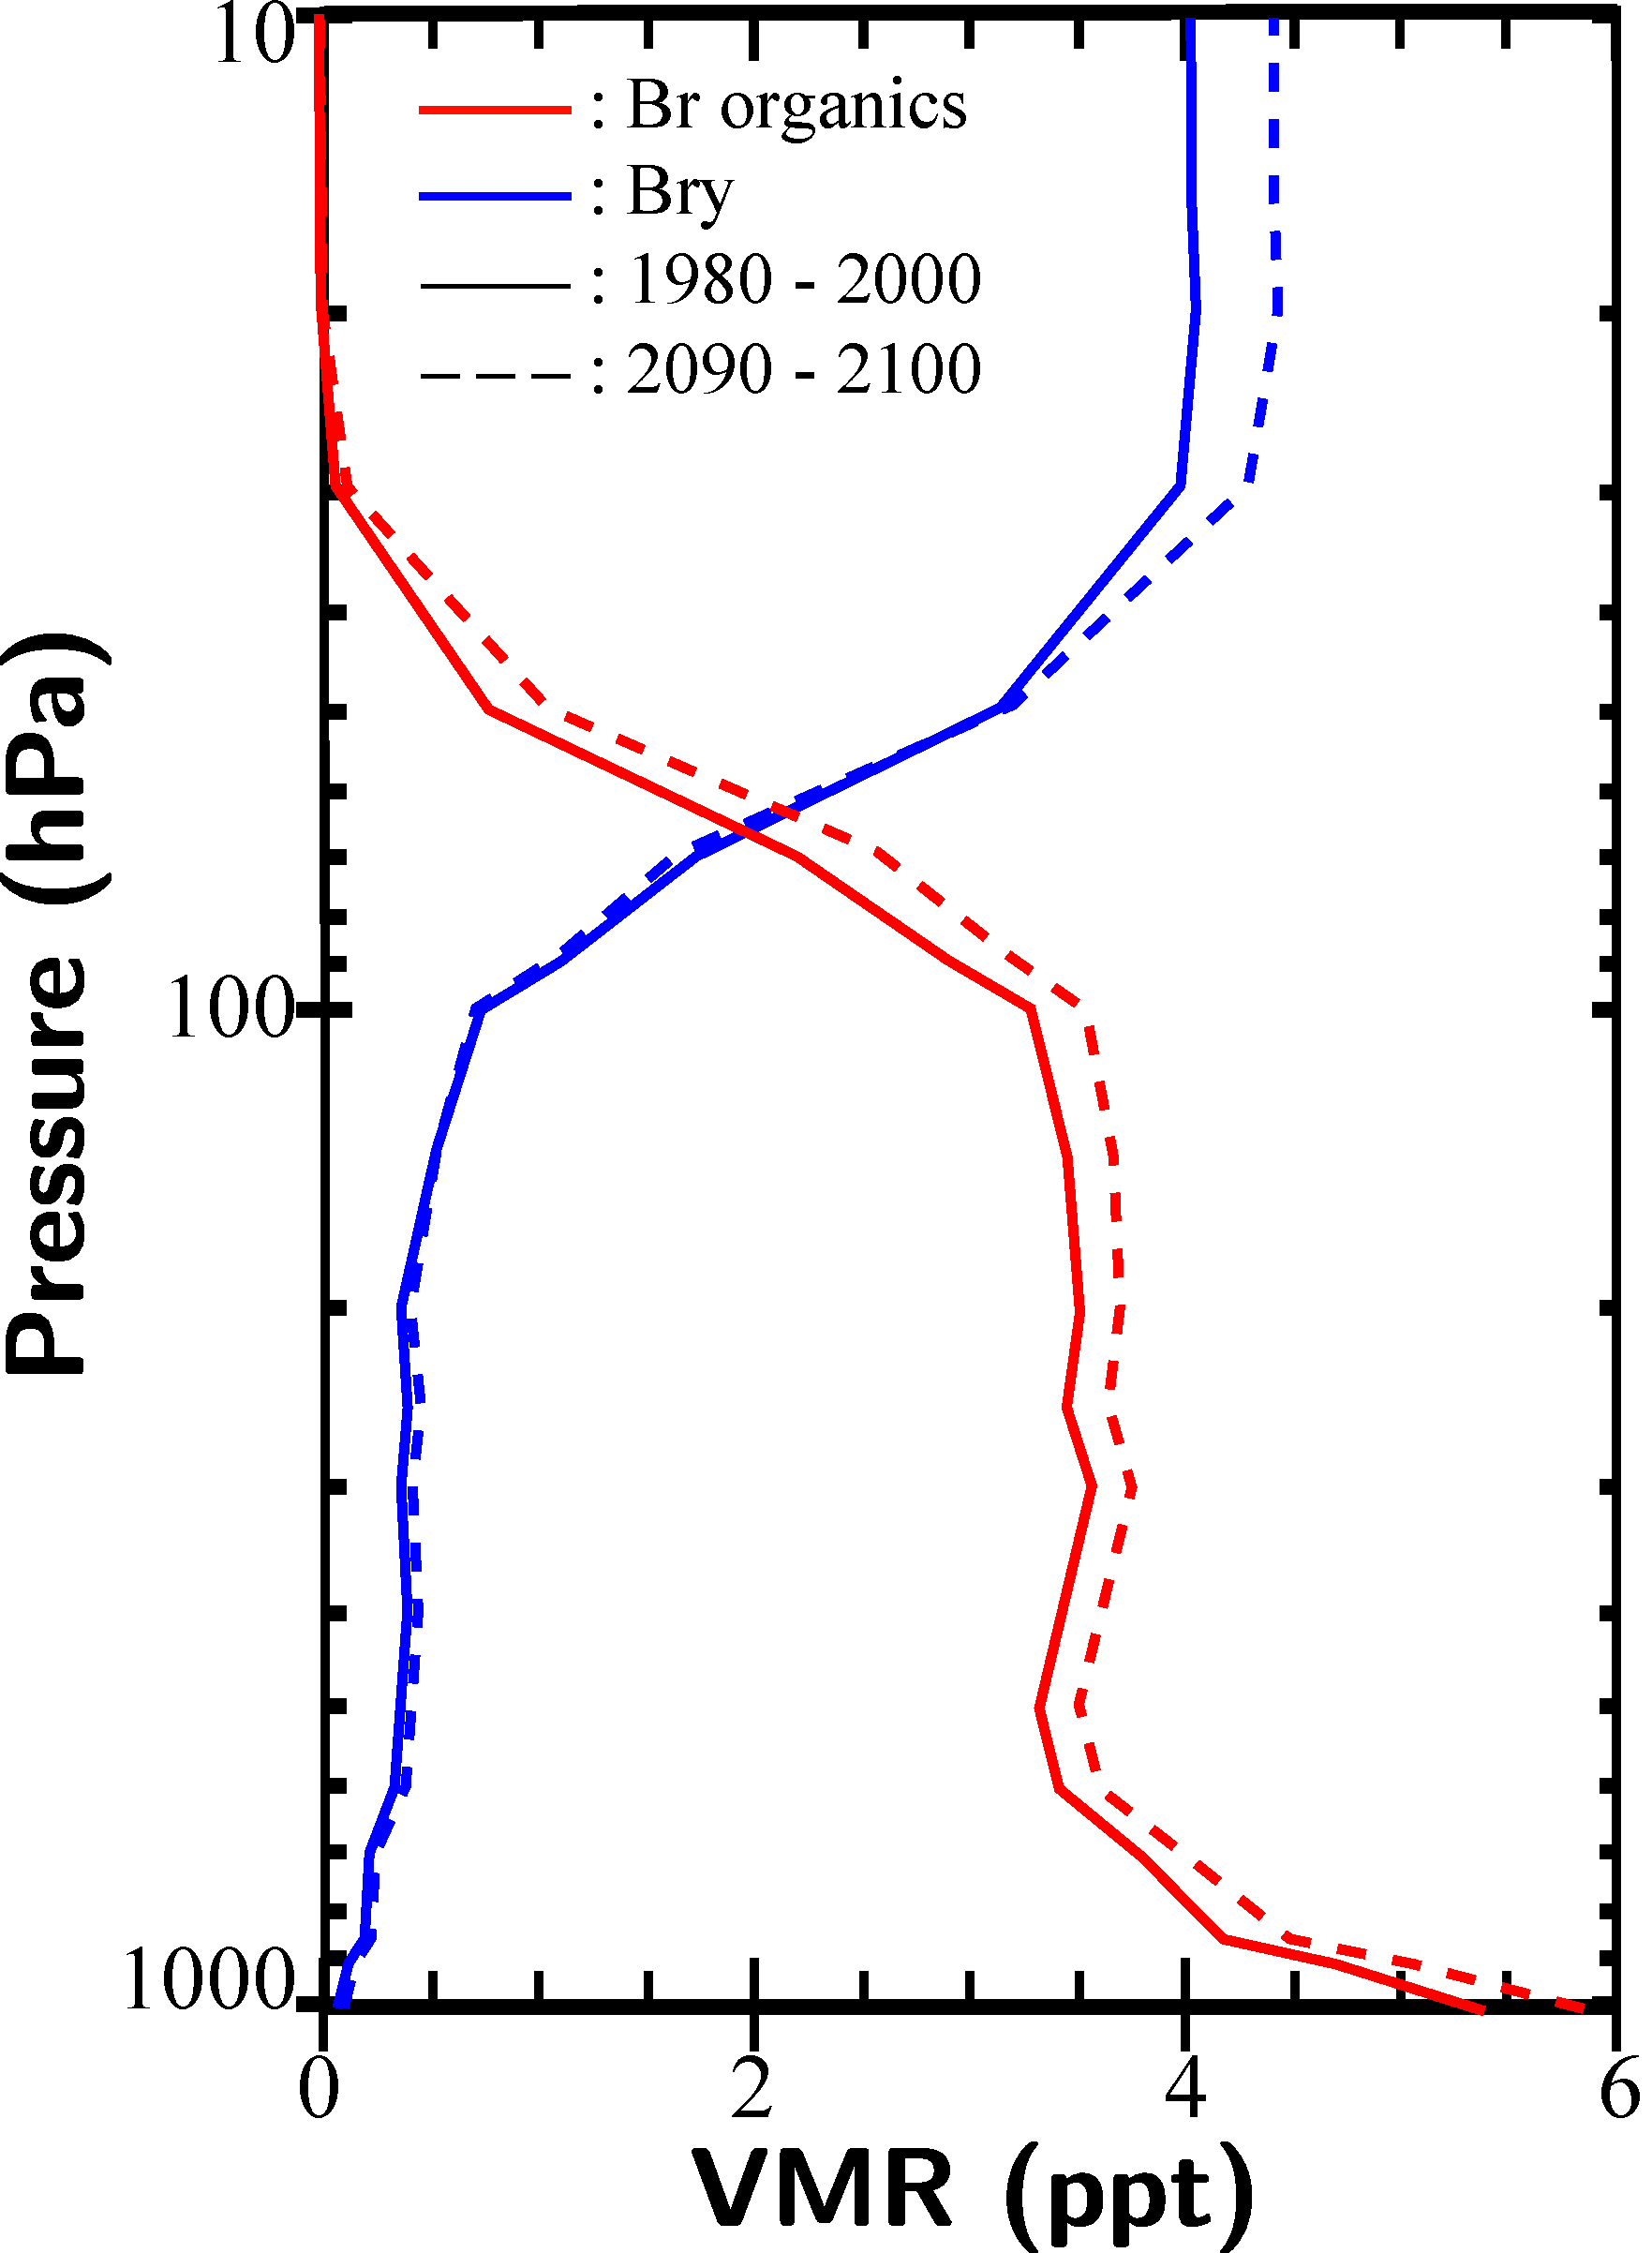
\includegraphics[width=8.3cm]{fig04}
  \caption[]{Tropical zonal mean (20$^\circ$~N--20$^\circ$~S), temporally averaged, vertical profiles of organic (\chem{Br_{org}}) and inorganic bromine (\chem{Br_y}) for the time periods 1990--2000 and 2090--2100 from SC\_free. In consistency with increasing VSLS fluxes \DIFdelbeginFL \DIFdelFL{(}\DIFdelendFL \DIFaddbeginFL \DIFaddFL{by }\DIFaddendFL 10\% \DIFdelbeginFL \DIFdelFL{)}\DIFdelendFL \DIFaddbeginFL \DIFaddFL{in the tropics}\DIFaddendFL , an increase of roughly 10\% in \chem{Br_y} from VSLS in the stratosphere is found, while the increase in \chem{Br_{org}} amounts to 8\%.}
  \label{fig:gisele-vsls-profiles}
\end{figure}
%
\section{Stratospheric bromine loading}
\label{sec:bromine_loading}
In addition to the possible increase in oceanic VSLS emissions due to climate change, discussed in the previous section, atmospheric transport and chemical transformation processes are also sensitive to climate change and may contribute to a change in the future stratospheric bromine loading from VSLS. These aspects will be studied in this section, based on the RC2-base-05 ESCiMo simulation, spanning 150 years from 1950 to 2100, assuming constant VSLS fluxes. Hence the fluxes of VSLS do not response to changes in the ground level abundances of VSLS.\\
%
In Fig.~\ref{fig:annual_mean_change_vsls}, profiles of brominated substances are shown for the tropics. The profiles are weighted by the amount of bromine atoms per molecule. The whole 150 year data set has been smoothed using a moving average with a box window size of 11 years to account for, e.g., seasonal variations, and the solar cycle. From these smoothed data, three reference years have been chosen for the analysis: 1980, 2016, and 2100. Therefore, 2100 is referring to June of the last valid year of the smoothed data (2094). To guide the eye, the corresponding mean tropical tropopause heights from the model output are shown together with the profiles. There is an upward shift of the tropopause height of about 8\,\unit{hPa} between present day and future. An upward shift of VSLS VMR profiles in 2100 in comparison to past/present day profiles is also visible. In the RCP6.0 scenario, ground level VMR of \chem{CH_3Br} and VSLS are constant from 2016 onward. In case of \chem{CH_3Br}, this roughly amounts to 1980 values. For all years, we find a fast decrease of VSLS of 5\,\unit{ppt} with a standard deviation of 0.25\,\unit{ppt} (or about 50\% compared to ground level VMR) between the surface and the mid-troposphere at about 500\,\unit{hPa}. The comparison of the difference of profiles between future and past/present (Fig.~\ref{fig:annual_mean_change_vsls}a, lower panel) reveals decreasing bromine values from VSLS by about 0.1--0.8\,\unit{ppt} throughout the troposphere, while there is an increase of the same order of magnitude in the lower stratosphere. Similar results have been published for RCP4.5 and RCP8.5 scenarios, attributing these to changes in the tropospheric circulation and to the primary oxidant \chem{OH}~\citep{GRL:Hossaini2012}. \DIFaddbegin \DIFadd{The amount of inorganic }\DIFaddend PG from VSLS (\chem{Br_y^{VSLS}}) \DIFdelbegin \DIFdel{, which have been traced within the simulation, are decreasing in the stratosphere in the future}\DIFdelend \DIFaddbegin \DIFadd{in the UTLS is decreasing by the same order of magnitude due to the enhanced upwelling in the tropics. As air in the UTLS becomes younger in a future climate, less SG (}\chem{Br_{org}^{VSLS}}\DIFadd{) will be dissociated into PG (}\chem{Br_y^{VSLS}}\DIFadd{) compared to present day}\DIFaddend . For 2016, this decline is compatible with a decreasing amount of VSLS in the troposphere. A slight excess of \chem{Br_y^{VSLS}} \DIFdelbegin \DIFdel{compared to 2016 and 2100 }\DIFdelend \DIFaddbegin \DIFadd{in the stratosphere }\DIFaddend is found for 1980 in \DIFdelbegin \DIFdel{the stratosphere. }\DIFdelend \DIFaddbegin \DIFadd{comparison to 2016 and 2100. }\DIFaddend This excess and the strong variability (denoted by the shown standard deviation) can be attributed to the hindcast period (1950--2005) of the simulation including volcanic eruptions. Large volcanic eruptions can influence the transport of bromine from VSLS into the stratosphere which may be related to a similar effect as seen in stratospheric water vapor~\citep{ACP:Loeffler2016}. Since volcanic activity has not been included in the future scenario, there is no such impact on \chem{Br_y^{VSLS}} from 2005 onward.\\
%
The largest change between present and future stems from the estimated decrease of long-lived SG, in particular Halons and \chem{CH_3Br}. At present, Halons contribute about 6--7\,\unit{ppt} to the total bromine loading of the lower stratosphere ($\sim$23\,\unit{ppt}), which is about the same amount as VSLS and \chem{CH_3Br} in RC2-base-05, whereas by the end of the century their contribution is reduced significantly to 1--2\,\unit{ppt} of total bromine ($\sim$17\,\unit{ppt}). This decline in long-lived, anthropogenically emitted SG is altering the amount of bromine released in the stratosphere on longer time scales. VSLS are already reduced due to photochemical dissociation when entering the TTL, while Halons are dissociating more slowly, providing a long lasting source of bromine to the stratosphere (Fig.~\ref{fig:annual_mean_change_vsls}b, lower panel). It is important to note, that although there is an \DIFdelbegin \DIFdel{apparent }\DIFdelend increase of \chem{Br_{org}^{VSLS}} of 0.5\,\unit{ppt} in the stratosphere assuming constant ocean--atmosphere fluxes, the overall amount of bromine in the stratosphere due to VSLS \DIFdelbegin \DIFdel{is }\DIFdelend \DIFaddbegin \DIFadd{(}\chem{Br_{tot}^{VSLS}}\DIFadd{) might be }\DIFaddend decreasing in the future. \DIFaddbegin \DIFadd{This depends on whether PG (}\chem{Br_y^{VSLS}}\DIFadd{) are transported alongside the VSLS into the UTLS or removed through washout in the troposphere. The model representations of underlying processes, e.g., conversion between soluble and insoluble inorganic bromine species through heterogeneous chemical reactions, are still uncertain.}\DIFaddend \\
%
In the following, we will derive a semi-analytic model to separate various aspects affecting the future VSLS distribution in the atmosphere (Section~\ref{subsec:local_lifetime}). Since the atmospheric window for air entering the stratosphere is located in the tropics, we will focus on averaged tropical atmospheric quantities. Subsequently, the transition between troposphere and stratosphere caused by a rising tropopause is influencing the interpretation of VMR profile differences between present and future. This will be discussed in Section~\ref{subsec:tropopause}.
%
\begin{figure*}[t]
  \centering
  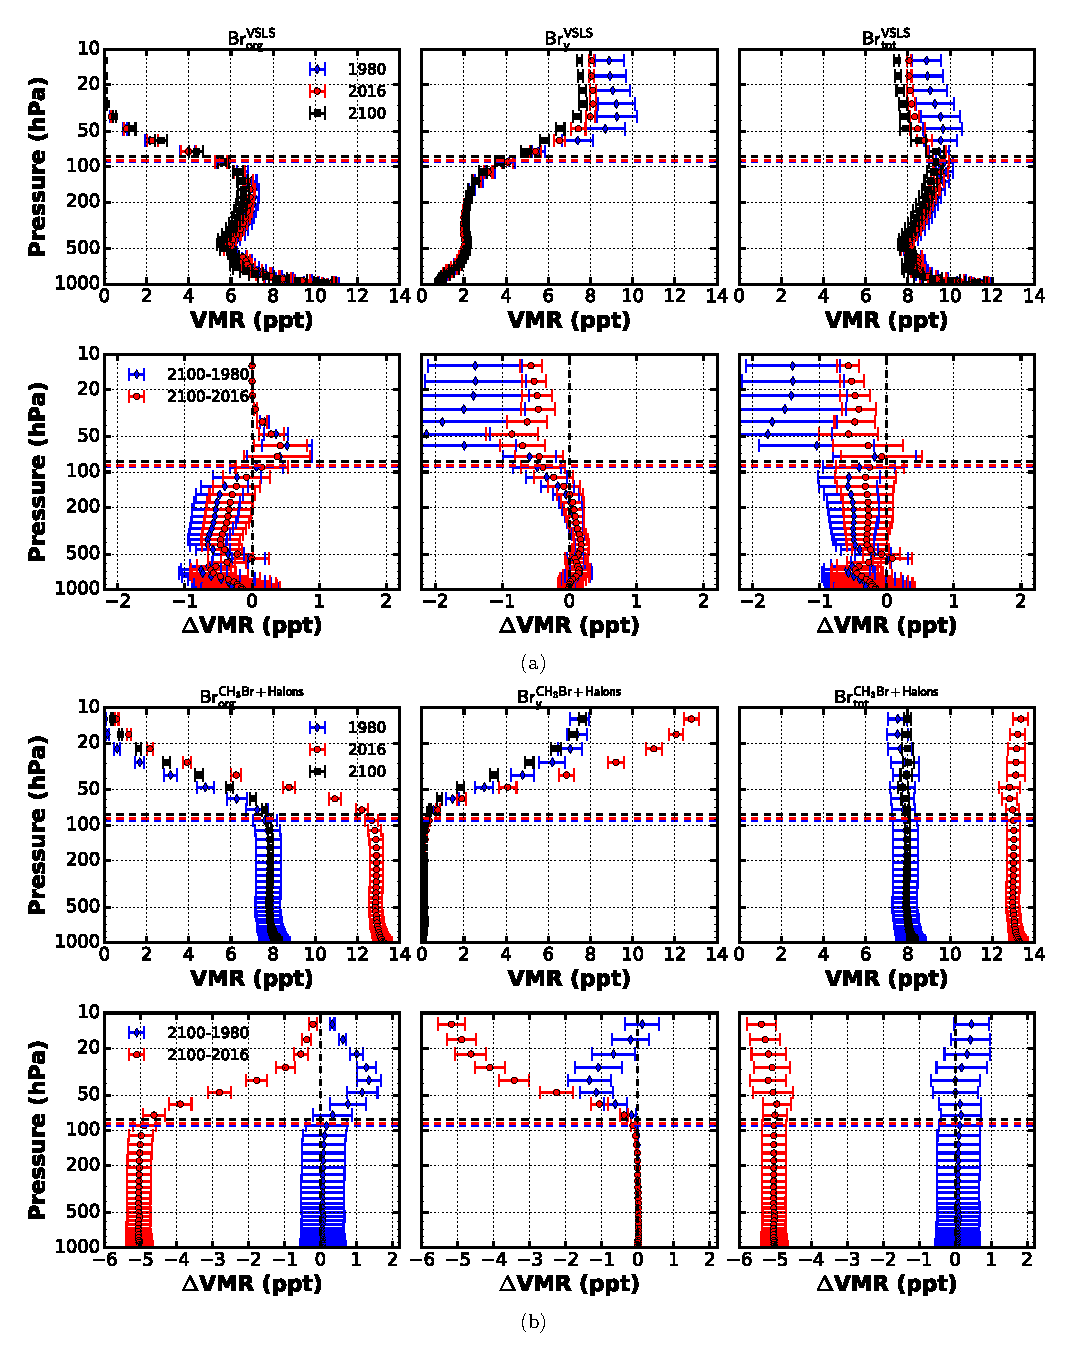
\includegraphics[width=12cm]{fig05} 
  \caption[]{Vertical profiles of brominated substances divided into SG (\chem{Br_{org}}), PG (\chem{Br_y}), and SG + PG (\chem{Br_{tot}}) in the tropics (20$^\circ$~N--20$^\circ$~S). Data from ESCiMo RC2-base-05 simulation~\citep{GMD:Joeckel2016}. Absolute values of VMR in upper panel, difference $\Delta$VMR with respect to 2100 values in lower panel. (a) Bromine from VSLS; (b) Bromine from \chem{CH_3Br} and Halons.}
  \label{fig:annual_mean_change_vsls}
\end{figure*}
%
%\begin{figure*}[t]
%  \centering
%  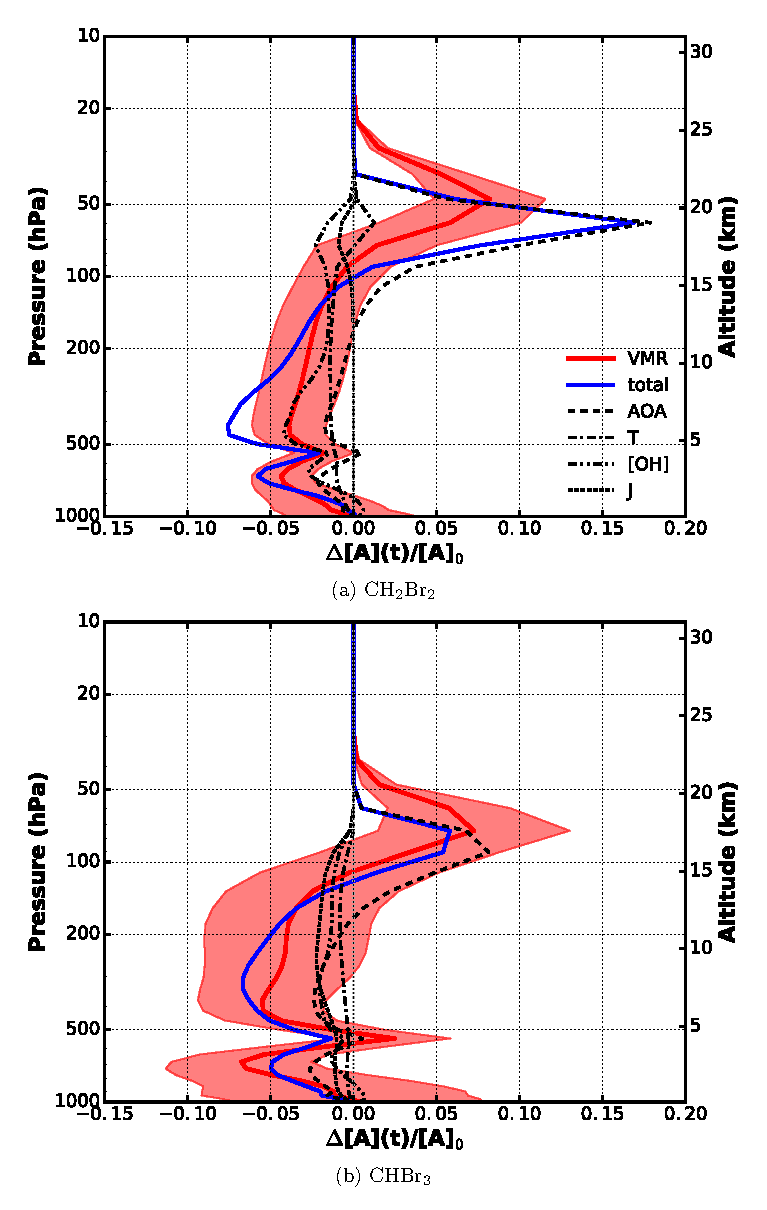
\includegraphics[width=12cm]{fig07}
%  \caption[]{VMR profiles of bromine from organic brominated source gases and total of bromine from inorganic product gases for past (1980), present (2016), and future (2100). Species have been scaled according to their amount of bromine.}
%  \label{fig:rc2-base-05-all_profiles}
%\end{figure*}
%
\subsection{Quantification of future atmospheric changes affecting VSLS mixing ratio profiles}
\label{subsec:local_lifetime}
The increase of VSLS in the stratosphere in the future can be attributed to changes in chemical and photolytical dissociation rates, and alternating transport from source regions through the TTL caused by a speed-up of the Brewer--Dobson circulation~(BDC)~\citep{GRL:Hossaini2012}.  
All of these factors influence the lifetime of VSLS in the atmosphere. A volume of air in a certain height (or rather pressure coordinate) shall have an associated mean temperature $T$, \chem{OH} concentration [\chem{OH}], photolysis frequency $J$, and age of air~(AOA). 
In the model, VSLS are dissociated photochemically via
%
\begin{reaction}
  \label{reac:oxi_CH2Br2}
  \chem{CH_2Br_2} + \chem{OH} \rightarrow \chem{2Br} + \chem{H_2O},
\end{reaction}
%
\begin{reaction}
  \label{reac:oxi_CHBr3}
  \chem{CHBr_3} + \chem{OH} \rightarrow \chem{3Br} + \chem{H_2O},
\end{reaction}
and 
\begin{reaction}
  \label{reac:photo_CH2Br2}
  \chem{CH_2Br_2} + h\nu \rightarrow \chem{2Br} + \chem{products},
\end{reaction}
%
\begin{reaction}
  \label{reac:photo_CHBr3}
  \chem{CHBr_3} + h\nu \rightarrow \chem{3Br} + \chem{products}.
\end{reaction}
The simplification in these equations compared to reality is justified since the intermediate reaction products \chem{CBr_2O} and \chem{CHBrO} insignificantly amount to the total bromine PG~\citep{ACP:Hossaini2010}.
From the resulting first order differential equation
%
\begin{equation}
  \label{eq:kin_gas}
  \frac{\mathrm{d[A]}}{\mathrm{d} t} = -k_\mathrm{A}(T)\cdot [\chem{OH}]\cdot \mathrm{[A]} - J_\mathrm{A} \cdot \mathrm{[A]},
\end{equation}
%
with [A] any of the VSLS species concentration, $k_\mathrm{A}(T)$ the temperature dependent rate coefficient, $J_\mathrm{A}$ the photolysis frequency~\citep{JPL_11-10}, and assuming [\chem{OH}] is unchanged by the reaction, a simple solution of Eq.~(\ref{eq:kin_gas}) is derived
%
\begin{align}
  \label{eq:reaction_rate}
  \mathrm{[A]}(t) &= \exp\left(-(k_\mathrm{A}(T)\cdot [\chem{OH}] + J_\mathrm{A})\cdot (t-t_0)\right)\cdot \mathrm{[A]}_0.
\end{align}
%
Based on above equation, the influence of [\chem{OH}], temperature, transport, and photolysis rate can be studied. For inferring the change in chemical dissociation, 10 year average profiles of [\chem{OH}], and one year average profiles of temperature have been computed from RC2-base-05 data for present day (2016) and future (2100). The idea is to assess the effect of transport timescales ($t_0 \rightarrow t$) by using 10 year averages of mean AOA from RC2-base-05 data (neglecting the age spectrum in the described volume of air). AOA shall refer to the time since an air parcel has been in contact with ground level. It has been evaluated in the EMAC simulation from an artificial, passive tracer with linearly increasing emission. Photolysis frequencies have been computed from averaged tropical profiles of temperature, humidity, and ozone column using the column version of \texttt{jval}~\citep{GMD:Sander2014} from EMAC. In case of photolysis frequencies, temperature dependence will not be discussed separately.\\ 
%
In Fig.~\ref{fig:changing_parameters}\DIFaddbegin \DIFadd{a}\DIFaddend , averaged profiles of temperature, AOA, and [\chem{OH}] are shown. Mean tropospheric temperatures are higher, while stratospheric temperatures are lower in the future, which is in line with other studies \DIFdelbegin \DIFdel{~\mbox{%DIFAUXCMD
\citep[see][Chap. 12]{IPCC2013}}%DIFAUXCMD
}\DIFdelend \DIFaddbegin \DIFadd{(e.g., \mbox{%DIFAUXCMD
\citet[][Chap. 12]{IPCC2013}}%DIFAUXCMD
, \mbox{%DIFAUXCMD
\citet[][Chap.2]{WMO2014}}%DIFAUXCMD
)}\DIFaddend . The concentration of \chem{OH} is increased throughout the atmosphere, apart from the lowermost levels. AOA will become notably younger within the stratosphere by the end of the century, as shown in various other studies~\citep{TAS:Austin2007,JC:Austin2013,CD:Butchart2006,JC:Li2008,GRL:Muthers2016}, and become slightly older (by a few days) in the troposphere. \DIFaddbegin \DIFadd{Vertical profiles of the }\chem{CHBr_3} \DIFadd{lifetime for present and future are shown in Fig.~\ref{fig:changing_parameters}b. Because of an increase in photolysis rates due to increasing temperatures, the }\chem{CHBr_3} \DIFadd{lifetime is decreasing. }\chem{CH_2Br_2} \DIFadd{is not shown, since its lifetime with respect to photolysis is almost infinite in the troposphere and thus determined by reaction with }\chem{OH}\DIFadd{.}\DIFaddend \\
%
By varying the variables in Eq.~(\ref{eq:reaction_rate}) one by one, the impact of each on the resulting profile difference ($\mathrm{\Delta[A]}(t)/\mathrm{[A]_0}$) has been calculated (Fig.~\ref{fig:changing_profiles}). The increase of [\chem{OH}] in the RCP6.0 scenario results in a general decreasing VMR of VSLS in the troposphere and lower stratosphere. The influence is highest at 500\,\unit{hPa} and around the tropopause. \chem{CH_2Br_2} is affected more strongly by a change of [\chem{OH}] due to chemical destruction ($\sim$5\%) than \chem{CHBr_3} ($\sim$2\%). The change in mean temperatures causes a tropospheric VMR decrease by at most 2\%. In the stratosphere decreasing temperatures increase $\mathrm{\Delta[A]}(t)/\mathrm{[A]_0}$ by about 1\%.
An increased AOA in the troposphere is reflected by a decreasing $\mathrm{\Delta[A]}(t)/\mathrm{[A]_0}$ ($\sim$2\%), while the opposite is true for the juvenescence of air in the stratosphere (8--18\%). For \chem{CH_2Br_2}, the impact of AOA is apparently overestimated in the lower stratosphere by this ansatz, which might be because of the neglected AOA spectrum representing a mixing of different air masses. Since the photolytical lifetime of \chem{CH_2Br_2} in the troposphere is infinite, it has no influence on the tropospheric part of the profile. A weak decrease in the order of 1--2\% is apparent in the lower stratosphere. This has been found to be mainly driven by temperature sensitivity of photolysis. In case of \chem{CHBr_3}, a 1--2\% decrease due to changing photolysis is found in the free and upper troposphere. This change in photolysis rate is mainly due to changes in tropical ozone abundance.\\
If all occurring changes are included, the actual profile differences between future and present are rather well reproduced (shown in red). These VMR profiles are 10 year averages for the tropics. The corresponding standard deviation is plotted as shaded error band. The decreasing VMR of VSLS in the troposphere is in the order of 5--7\% (at about 250\,\unit{hPa}) for \chem{CH_2Br_2} and \chem{CHBr_3}, respectively. In the stratosphere, the maximum increase, dependent on specie, occurs at differing pressure levels and amounts to 7--8\%.\\
In Summary, all occurring future changes are decreasing VMR of VSLS in the troposphere. In case of \chem{CHBr_3}, all factors are of the same order of magnitude. The tropospheric decrease of \chem{CH_2Br_2} VMR is mainly driven by increasing [\chem{OH}]. In the upper troposphere / lower stratosphere~(UTLS), the impact of the juvenescence of AOA dominates, inflicting an increase in VMR.
%
\begin{figure}[t]
  \centering
  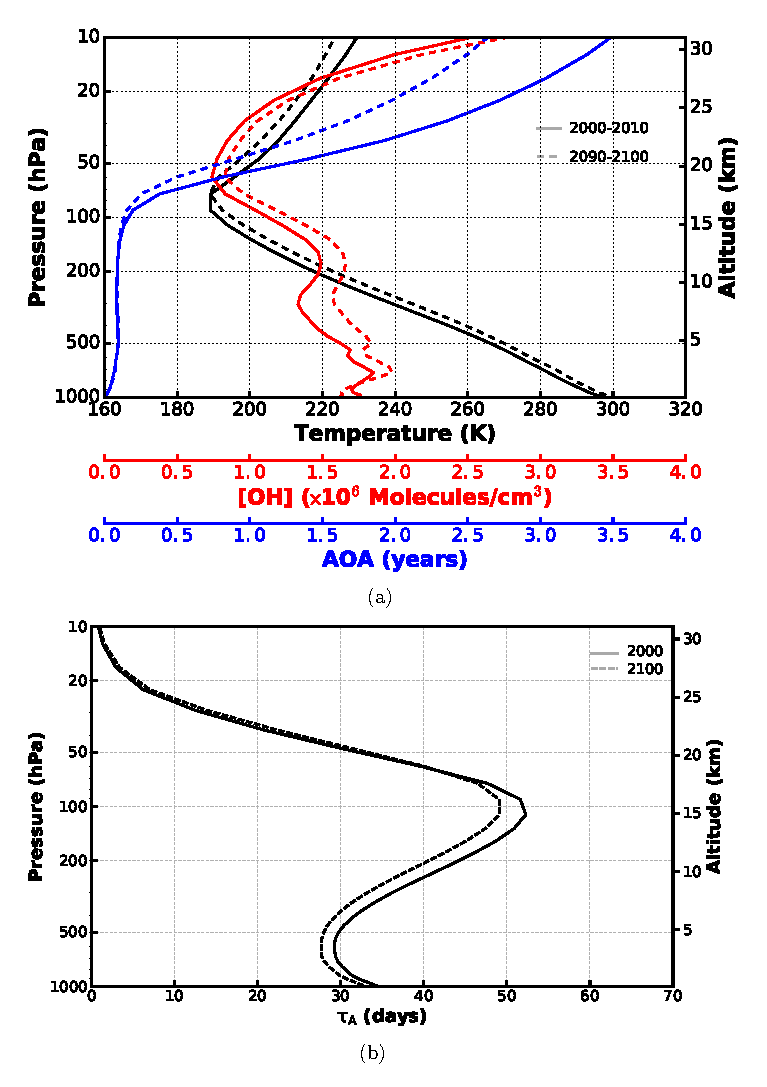
\includegraphics[width=8.3cm]{fig06}
  \caption[]{Tropical average profiles from ESCiMo RC2-base-05 simulation of changing variables in Eq.~(\ref{eq:reaction_rate}) for present day (solid lines) and future (dashed lines). \DIFaddbeginFL \DIFaddFL{(a) Temperature, OH concentration, and age of air; (b) Lifetime of }\chem{CHBr_3}\DIFaddFL{.}\DIFaddendFL } 
  \label{fig:changing_parameters}
\end{figure}
%
%\begin{figure}[t]
%  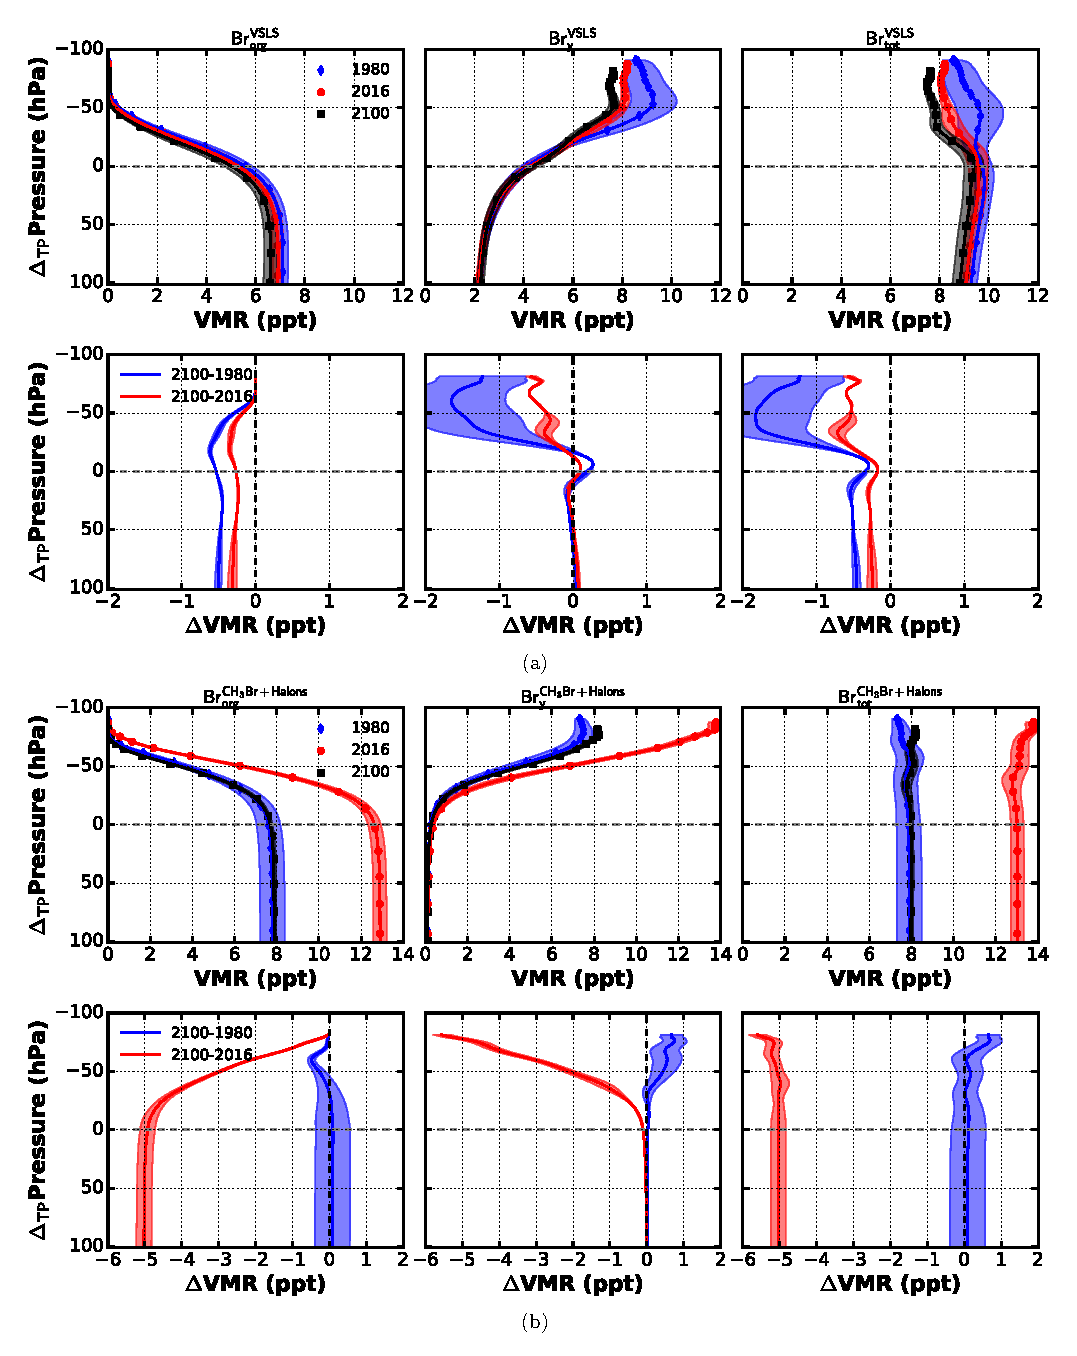
\includegraphics[width=8.3cm]{fig09}
%  \caption[]{Difference in tropospheric AOA between future and present. Tropical average profiles from ESCiMo RC2-base-05 simulation. Monthly means in gray, annual mean in blue.} 
%  \label{fig:delta_aoa_tropics_troposphere}
% \end{figure}
%
%\begin{figure}[t]
%  \centering
%  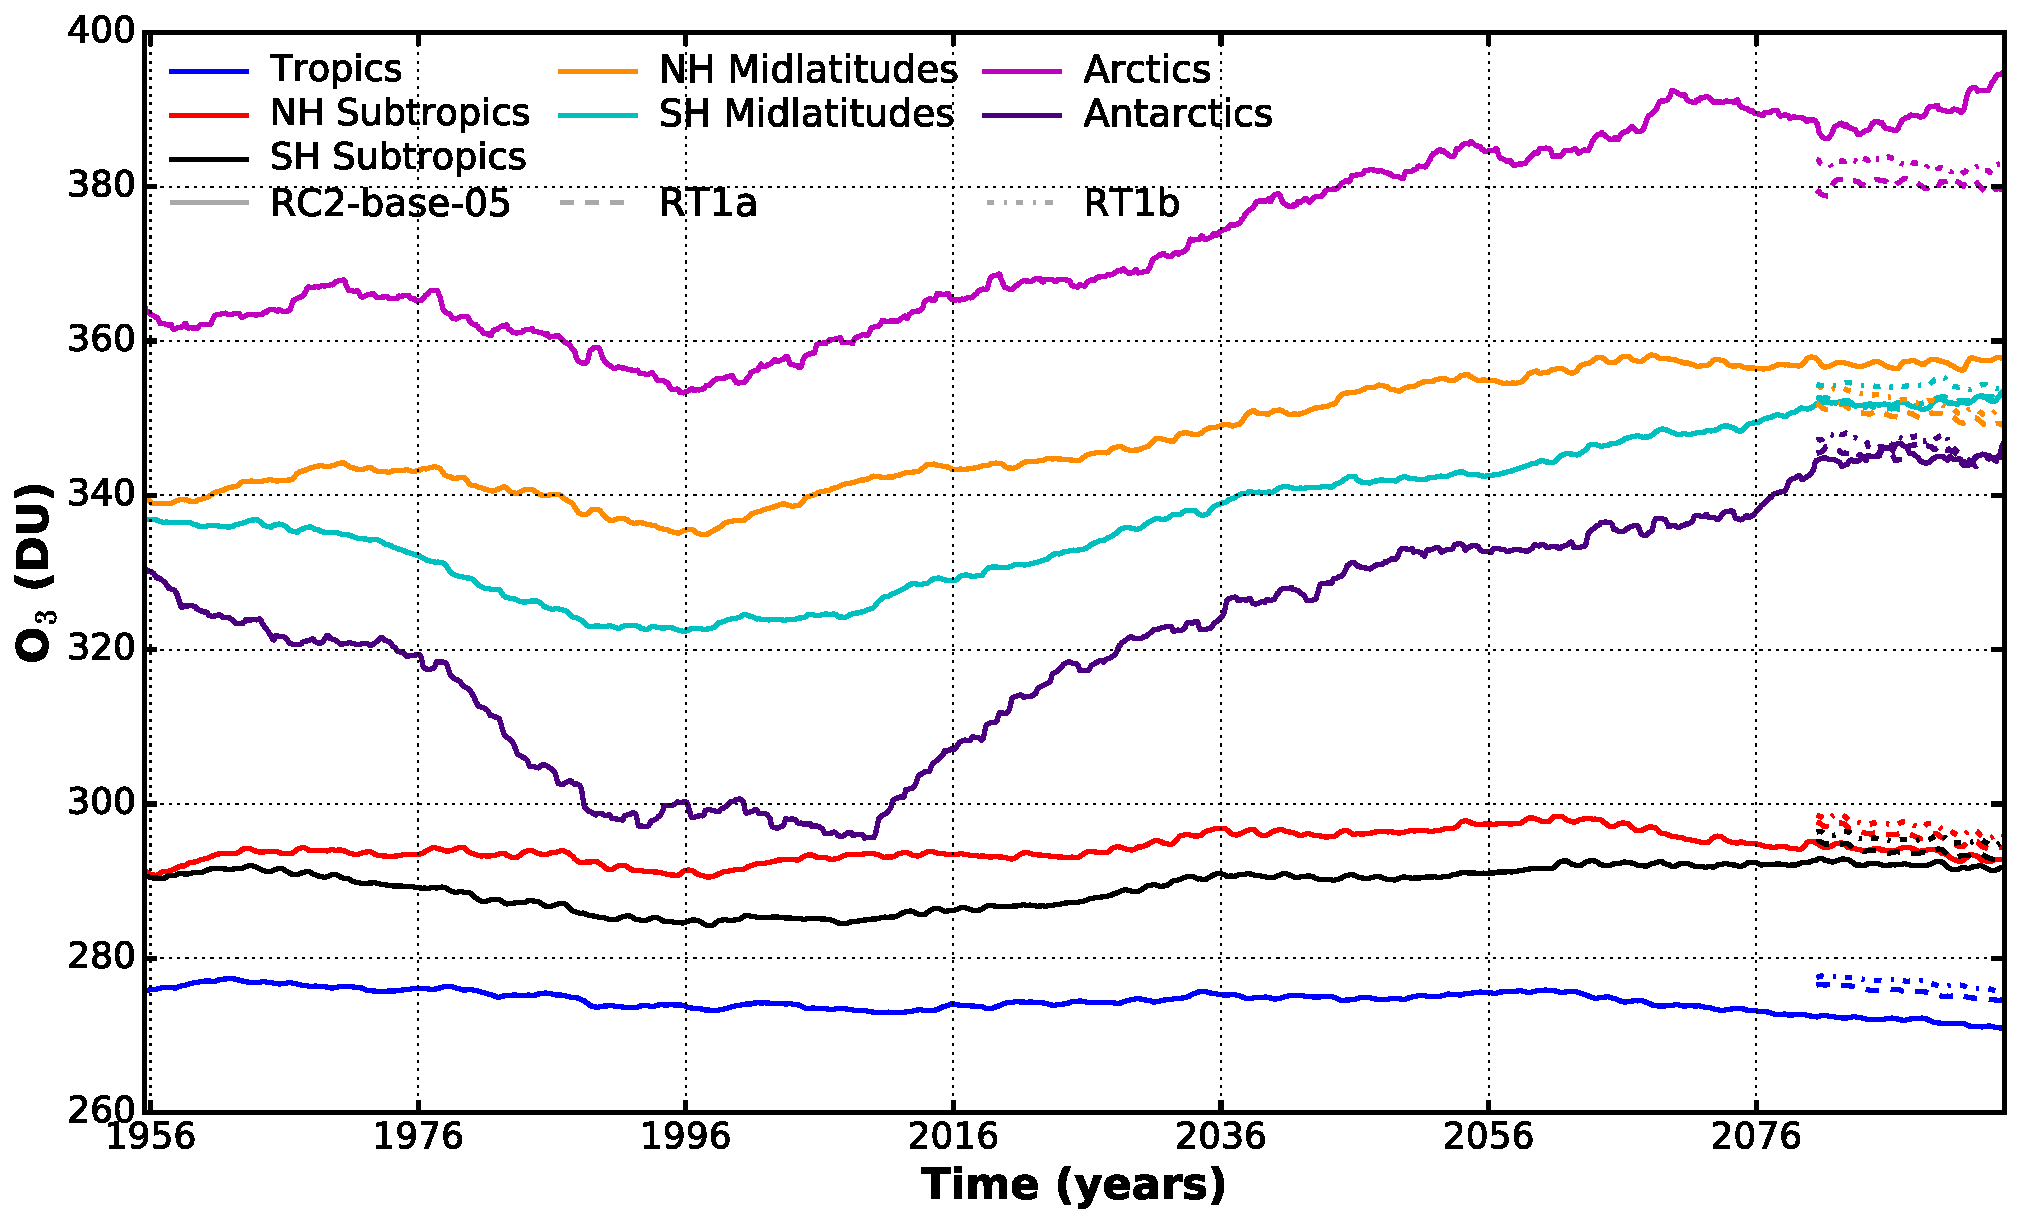
\includegraphics[width=8.3cm]{fig10}
%DIF <   \caption[]{Average lifetime of VSLS species $\tau_\mathrm{A}$ due to photolysis for solar zenith angles ranging from 0--90$^\circ$. The average daily lifetime has been inferred from an area weighted mean and accounting for absent photolysis at night times.}
%DIF >   \caption[]{Average lifetime of VSLS species $\tau_\text{A}$ due to photolysis for solar zenith angles ranging from 0--90$^\circ$. The average daily lifetime has been inferred from an area weighted mean and accounting for absent photolysis at night times.}
%  \label{fig:vsls_lifetimes}
%\end{figure}
%
\begin{figure}[t]
  \centering
  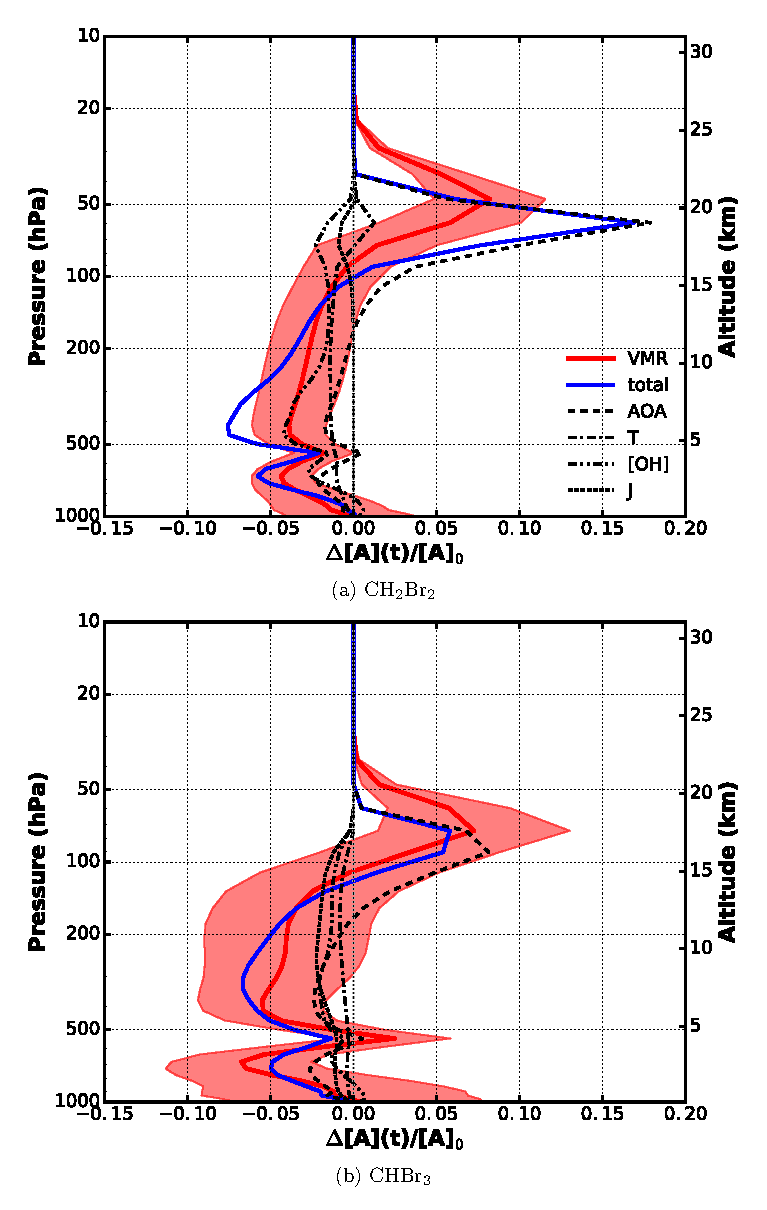
\includegraphics[width=8.3cm]{fig07}
  \caption[]{Relative difference of VSLS vertical profiles for 2000 and 2100. Major influences on lifetime have been separated.Shown are resulting profiles by varying the denoted variables, mean temperature $T$, \chem{OH} concentration [\chem{OH}], photolysis frequency $J$, and age of air~(AOA), in Eq.~(\ref{eq:reaction_rate}) one by one.}
  \label{fig:changing_profiles}
\end{figure}
%
\subsection{Implications of a rising tropopause on VSLS mixing ratio profiles}
\label{subsec:tropopause}
The GHG induced warming of the troposphere and cooling of the stratosphere causes a rise of the tropopause. Model mean tropical tropopause heights from RC2-base-05 have been smoothed using a moving average with a box window size of 11 years. The corresponding standard deviation is displayed as yellow band in Fig.~\ref{fig:tropopause}. A linear regression fit on the smoothed model mean tropical tropopause height yields a rise of $(0.81\pm0.01)$\,\unit{hPa\,decade^{-1}}. This is in accordance with results from ECMWF Re-Analysis data for the past two decades~\citep{QJRMS:Wilcox2012}.  As indicated by~\citet{GRL:Oberlaender2016} regarding the BDC, the upward shift of the tropopause affects the interpretation of vertical profile differences between future and past. An air parcel which would have already entered the stratosphere under present day conditions may be still considered tropospheric in the future. As pointed out earlier, profiles appear shifted by a fraction of distance between two pressure coordinate levels. We perform a spline fit to the averaged profiles and shift them accordingly with respect to the mean tropopause. The fit results have been evaluated within a valid region of $\pm$100\,\unit{hPa} around the tropopause. The results are shown in Fig.~\ref{fig:annual_mean_change_relativ_tp}. Uncertainty bands have been estimated by adding/subtracting one standard deviation from the averaged VMR profiles and computing the corresponding splines. With respect to the mean tropopause, VMR differences show no increase of bromine from VSLS in the lower stratosphere, but rather a slight decrease (Fig.~\ref{fig:annual_mean_change_relativ_tp}a). A small increase of inorganic bromine from VSLS (\chem{Br_y^{VSLS}}) is found in the tropopause region. At about 20\,\unit{hPa}, \chem{Br_y^{VSLS}} is reduced by 1--2\,\unit{ppt} in the future compared to 1980. Overall, a reduction of bromine in the UTLS is found at the end of the 21st century. In Fig.~\ref{fig:annual_mean_change_relativ_tp}b, the amount of bromine from \chem{CH_3Br} and Halons is shown. Except for a slight increase of \chem{Br_{tot}^{CH_3Br+Halons}} in the upper stratosphere between 1980 and 2100 of about 0.7\,\unit{ppt}, there is no increase of bromine from long-lived SG.\\
To summarize, the \DIFdelbegin \DIFdel{main reason to the apparent increase of bromine from VSLS above 100\,}%DIFDELCMD < \unit{hPa} %%%
\DIFdelend \DIFaddbegin \DIFadd{increase of lower stratospheric VSLS }\DIFaddend in RC2-base-05 of about 5--10\% is \DIFdelbegin \DIFdel{the increase in }\DIFdelend \DIFaddbegin \DIFadd{due to enhanced }\DIFaddend vertical transport in the tropics. \DIFdelbegin \DIFdel{Although bromine loading from VSLS above 100\,}%DIFDELCMD < \unit{hPa} %%%
\DIFdel{isincreased at the end of the 21st century, the stratospheric abundance of }\DIFdelend \DIFaddbegin \DIFadd{This increase is, however, counteracted by a corresponding decrease in inorganic bromine. Everything else unchanged, an increase in tropical upwelling will therefore not change the total amount of bromine in the future stratosphere. Additionally, due to enhanced future }\chem{OH} \DIFadd{concentrations in RCP6.0, the tropospheric lifetime of VSLS is reduced which leads to a decrease of total }\DIFaddend bromine from VSLS\DIFdelbegin \DIFdel{is not increasing but decreasing by about 1--2\,}%DIFDELCMD < \unit{ppt}%%%
\DIFdel{, if }\DIFdelend \DIFaddbegin \DIFadd{. As mentioned in Section~\ref{sec:emission_trends}, whether the amount of inorganic PG in the UTLS is decreasing or not, strongly depends on the partitioning of }\chem{Br_y} \DIFadd{and conversion of soluble }\chem{HBr} \DIFadd{and }\chem{HOBr} \DIFadd{into insoluble }\chem{BrO} \DIFadd{through heterogeneous recycling, e.g., occurring on sea-salt aerosols or ice-crystals. In case insoluble species are favored, vertical transport would enhance the amount of PG in the UTLS. Otherwise, wet removal in the troposphere would decrease the amount of PG. This mechanism has not been explicitly tested in our model simulations.
Taken }\DIFaddend an upward shift of the tropopause \DIFdelbegin \DIFdel{is taken into consideration }\DIFdelend \DIFaddbegin \DIFadd{into consideration and shifting the VMR profiles accordingly with respect to the mean tropical tropopause height, a decrease of }\chem{Br_{tot}^{VSLS}} \DIFadd{by 0.5--2\,}\unit{ppt} \DIFadd{is found for a fixed $\Delta_\mathrm{TP}P \approx 20$\,}\unit{hPa}\DIFaddend .
%
\begin{figure}[t]
  \centering
  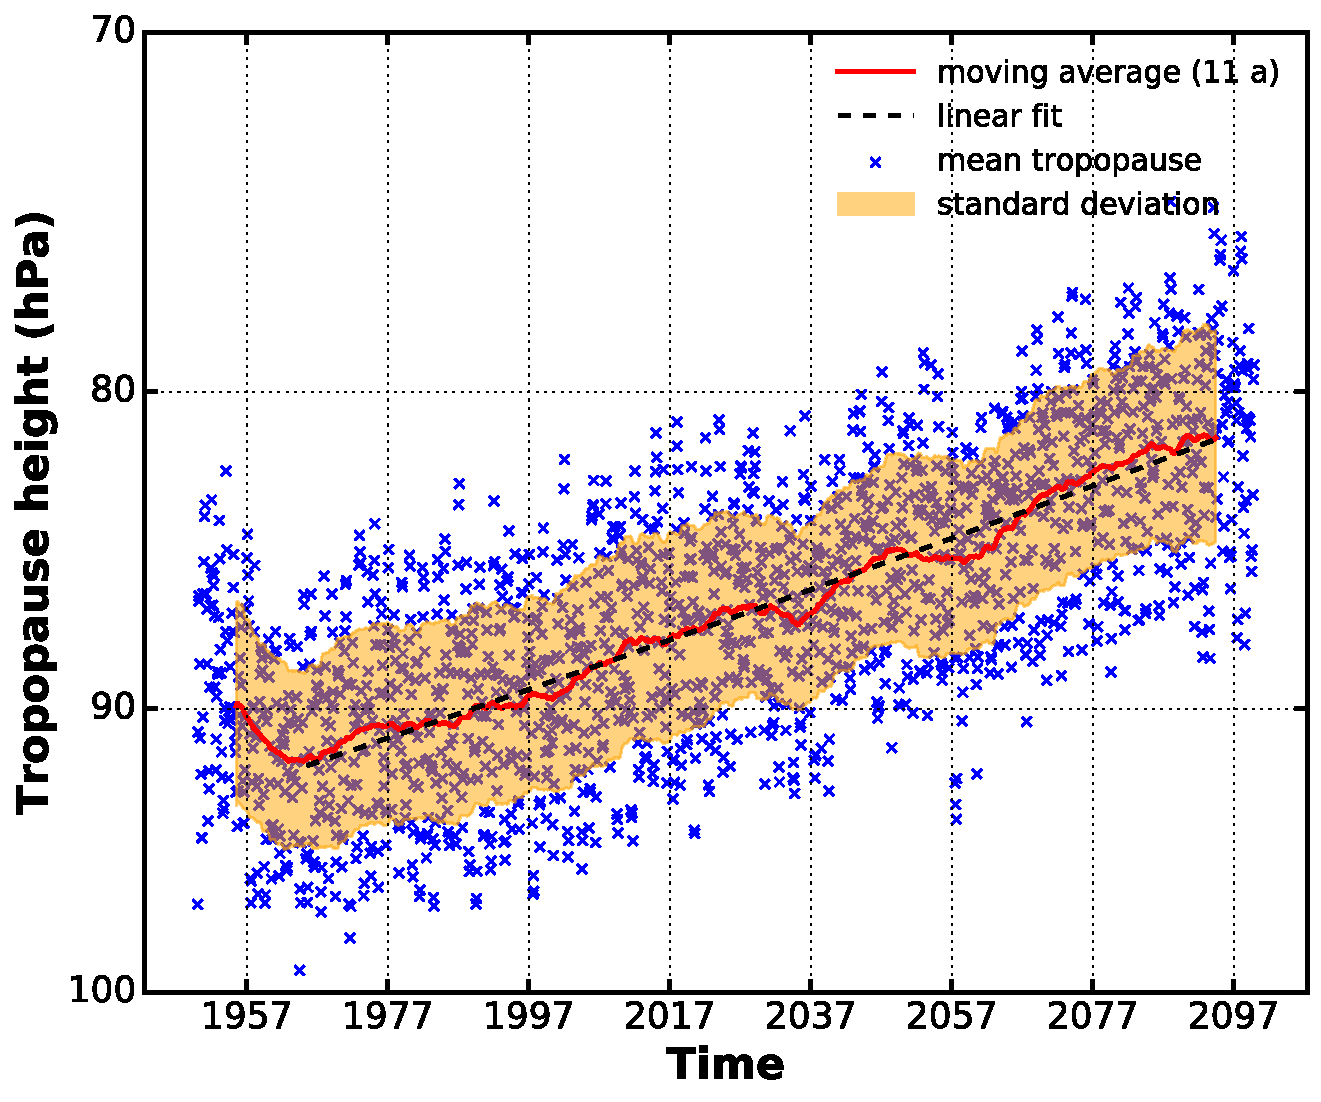
\includegraphics[width=8.3cm]{fig08}
  \caption[]{Model mean tropical tropopause from RC2-base-05 over a time span of 150 years. Tropopause data have been evaluated after the apparent spin-up of about 10 years. A rise of the mean tropical tropopause of $(0.81\pm0.01)$\,\unit{hPa\,decade^{-1}} is found by linear regression.}
  \label{fig:tropopause}
\end{figure}
%
\begin{figure*}[t]
  \centering
  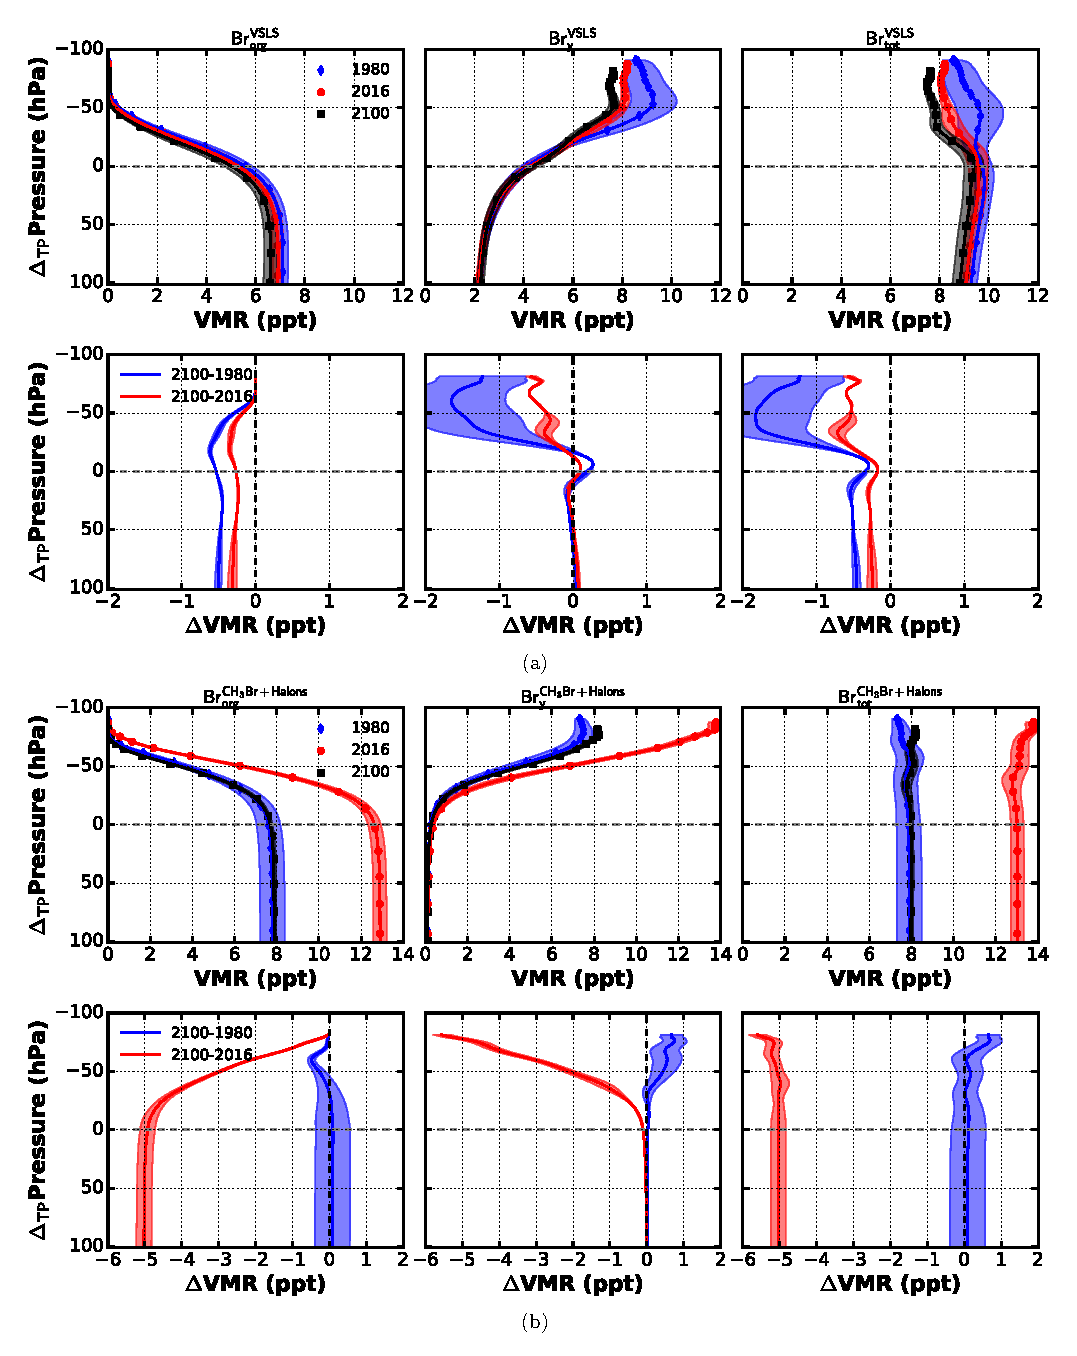
\includegraphics[width=12cm]{fig09} 
  \caption[]{Spline fitted vertical profiles of brominated substances divided into SG (\chem{Br_{org}}), PG (\chem{Br_y}), and SG + PG (\chem{Br_{tot}}) in the tropics (20$^\circ$N--20$^\circ$S) with respect to the mean tropical tropopause. Data from ESCiMo RC2-base-05 simulation~\citep{GMD:Joeckel2016}. Absolute values of VMR in upper panel, difference $\Delta$VMR with respect to 2100 values in lower panel. (a) Bromine from VSLS; (b) Bromine from \chem{CH_3Br} and Halons.}
  \label{fig:annual_mean_change_relativ_tp}
\end{figure*}
%
\section{Implications on ozone depletion}
\label{sec:ozone_depletion}
In this section, the influence of brominated very short-lived source gases on ozone depletion will be \DIFdelbegin \DIFdel{studied based }\DIFdelend \DIFaddbegin \DIFadd{discussed. Based }\DIFaddend on RT1a and RT1b\DIFaddbegin \DIFadd{, we assess the impact of VSLS on a zonally averaged ozone distribution at the end of the 21st century}\DIFaddend . For a thorough discussion of future trends, the 25 year data set is too short. \DIFdelbegin \DIFdel{Results }\DIFdelend \DIFaddbegin \DIFadd{However, from our long-term simulations (SC\_free, SC\_nudged, RC2-base-05), long-term influence of emission perturbations on ozone is not assessable. As described in Section~\ref{sec:model_exp}, SC\_free does not include interactive ozone chemistry, whereas RC2-base-05 incorporates prescribed fluxes based on scenario five by~\mbox{%DIFAUXCMD
\citet{JGR:Warwick2006}}%DIFAUXCMD
. Furthermore, results }\DIFaddend from RC2-base-05 cannot be compared to RT1a/RT1b directly, because of significant differences in ozone distribution and amount between the differing vertical resolutions (L47MA and L90MA) of the model. This issue has been already reported by~\citet{GMD:Joeckel2016}.\\ 
Zonally averaged data of total column ozone have been smoothed using a moving average algorithm with box window size of 11 years (Fig.~\ref{fig:Zonal_Total_Ozone}). In general, ozone trends at the end of the century are roughly the same for both resolutions. The actual amount of ozone differs, with L90 showing more ozone except for the northern hemisphere polar region and mid-latitudes. In the Arctic RT1a/RT1b even indicate, in contrast to RC2-base-05, slightly decreasing total column ozone. In case of RT1a/RT1b, this might be partially caused by interactive aerosol and accordingly added oceanic COS source. This bias in total column ozone between the vertical resolutions is larger than the difference between RT1a and RT1b.\\
%
For estimating the effect of brominated VSLS on ozone depletion, the difference in zonally averaged ozone of RT1a and RT1b has been computed. A period of 20 years (2080--2100) has been used accounting for an estimated model spin-up of five years in the beginning. In Fig.~\ref{fig:zonal_mean_ozone}, the relative difference ($\mathrm{(RT1a-RT1b)}/\mathrm{RT1a}\cdot100$) is shown as contour plot. Dashed lines indicate a decrease of ozone in the simulation with VSLS turned on (RT1a) compared to the one with VSLS turned off (RT1b), while solid lines indicate an increase. Significance has been estimated as divergence from zero in units of standard error of mean. It is indicated by shades of blue. \DIFdelbegin \DIFdel{The average tropopause is shown as red line. }\DIFdelend VSLS cause a tropospheric ozone reduction in the order of 1--2\%, mainly at high latitudes. The UTLS region in the tropics is most affected, there VSLS cause a decrease of ozone of about 3\%. The decrease of ozone in the high latitude troposphere and tropical UTLS is rendered significant. Increasing amounts of ozone ($\sim$1\%) are found in the Antarctic middle and upper stratosphere, but these are mainly not significant. This increase in ozone abundance may be due to dynamical \DIFdelbegin \DIFdel{feedbacks}\DIFdelend \DIFaddbegin \DIFadd{feedback}\DIFaddend ~\citep{ACP:Braesicke2013}.\\
%
\DIFaddbegin \DIFadd{While VSLS have a large impact on Antarctic ozone depletion during the Ozone Hole period, i.e. during times with high stratospheric chlorine loading from about the late 1970s to the second half of the 21st century (e.g. \mbox{%DIFAUXCMD
\citet{ACP:Fernandez2017}}%DIFAUXCMD
; \mbox{%DIFAUXCMD
\citet{GRL:Oman2016}}%DIFAUXCMD
; \mbox{%DIFAUXCMD
\citet{GRL:Sinnhuber2015}}%DIFAUXCMD
; \mbox{%DIFAUXCMD
\citet{ACP:Yang2014}}%DIFAUXCMD
), we find that by the end of the 21st century under low chlorine loading VSLS have less impact on total Antarctic stratospheric ozone depletion, although their importance relative to the total stratospheric halogene load is increasing (about 40\% in accordance to \mbox{%DIFAUXCMD
\citet{ACP:Fernandez2017}}%DIFAUXCMD
). Assuming an adherence to the Montreal protocol, stratospheric volume mixing ratios of }\chem{Cl_y} \DIFadd{will decrease exponentially in the course of the 21st century from its peak values in 2000. From the \mbox{%DIFAUXCMD
\citet[][Chap.2, Fig. 2--21]{WMO2014}}%DIFAUXCMD
, a decline of }\chem{Cl_y} \DIFadd{loading at 1\,}\unit{hPa} \DIFadd{of about 2\,}\unit{ppbv} \DIFadd{between 2000 and 2080 can be deduced. In accordance, we find a reduction of zonally averaged stratospheric }\chem{Cl_y} \DIFadd{at 1\,}\unit{hPa} \DIFadd{of 2.1\,}\unit{ppb} \DIFadd{by the end of the 21st century compared to year 2000 in RC2-base-05. Since RT1a/RT1b have identical chlorine load and do not include present day, we cannot assess the chlorine moderation effect from these two simulations. }\DIFaddend \citet{GRL:Sinnhuber2015} have shown a reduction of ozone due to VSLS in the TTL region in the order of 6\% during the period 1970--1982 with significantly less stratospheric chlorine compared to the later period 1983--2005 (7\%), while \DIFdelbegin \DIFdel{~}\DIFdelend \citet[Supplement][Fig.~S3]{NGS:Hossaini2015} show a change of total ozone column due to VSLS (on/off scenario) of the order of 1--3\% in pre-industrial conditions. Given that \DIFaddbegin \DIFadd{the VSLS emission }\DIFaddend scenario five of~\citet{JGR:Warwick2006} \DIFdelbegin \DIFdel{has about double }\DIFdelend \DIFaddbegin \DIFadd{used in RC2-base-05 has about twice }\DIFaddend the amount of VSLS compared to RT1a and chlorine abundance in the stratosphere will drop to 1970 values by the end of the 21st century~\citep[see][Chap. 12]{IPCC2013}, our results are in good agreement with these previous \DIFdelbegin \DIFdel{analysis}\DIFdelend \DIFaddbegin \DIFadd{studies}\DIFaddend . In more detail, \citet{ACP:Yang2014} investigated the \DIFaddbegin \DIFadd{combined }\DIFaddend influence of brominated VSLS \DIFdelbegin \DIFdel{in combination with differing levels of atmospheric chlorine load }\DIFdelend \DIFaddbegin \DIFadd{and chlorine }\DIFaddend on ozone. \DIFaddbegin \DIFadd{For two stratospheric }\chem{Cl_y} \DIFadd{loadings (3\,}\unit{ppb}\DIFadd{, 0.8\,}\unit{ppb}\DIFadd{), which correspond to 2000 and 2100, they have varied the amount of VSLS. \mbox{%DIFAUXCMD
\citet{ACP:Yang2014} }%DIFAUXCMD
have shown the more chlorine in the stratosphere the stronger ozone is affected by an increase of bromine VMR from VSLS. }\DIFaddend In concert with our results, although by doubling the initial amount of VSLS on a varying bromine background from anthropogenic sources, they have found a significant decrease of ozone in the tropical UTLS and polar region in the order of 2--4\% and slight, insignificant increases in the antarctic mid-stratosphere~\citep[Fig.~1e]{ACP:Yang2014}. 
%
\begin{figure}[t]
  \centering
  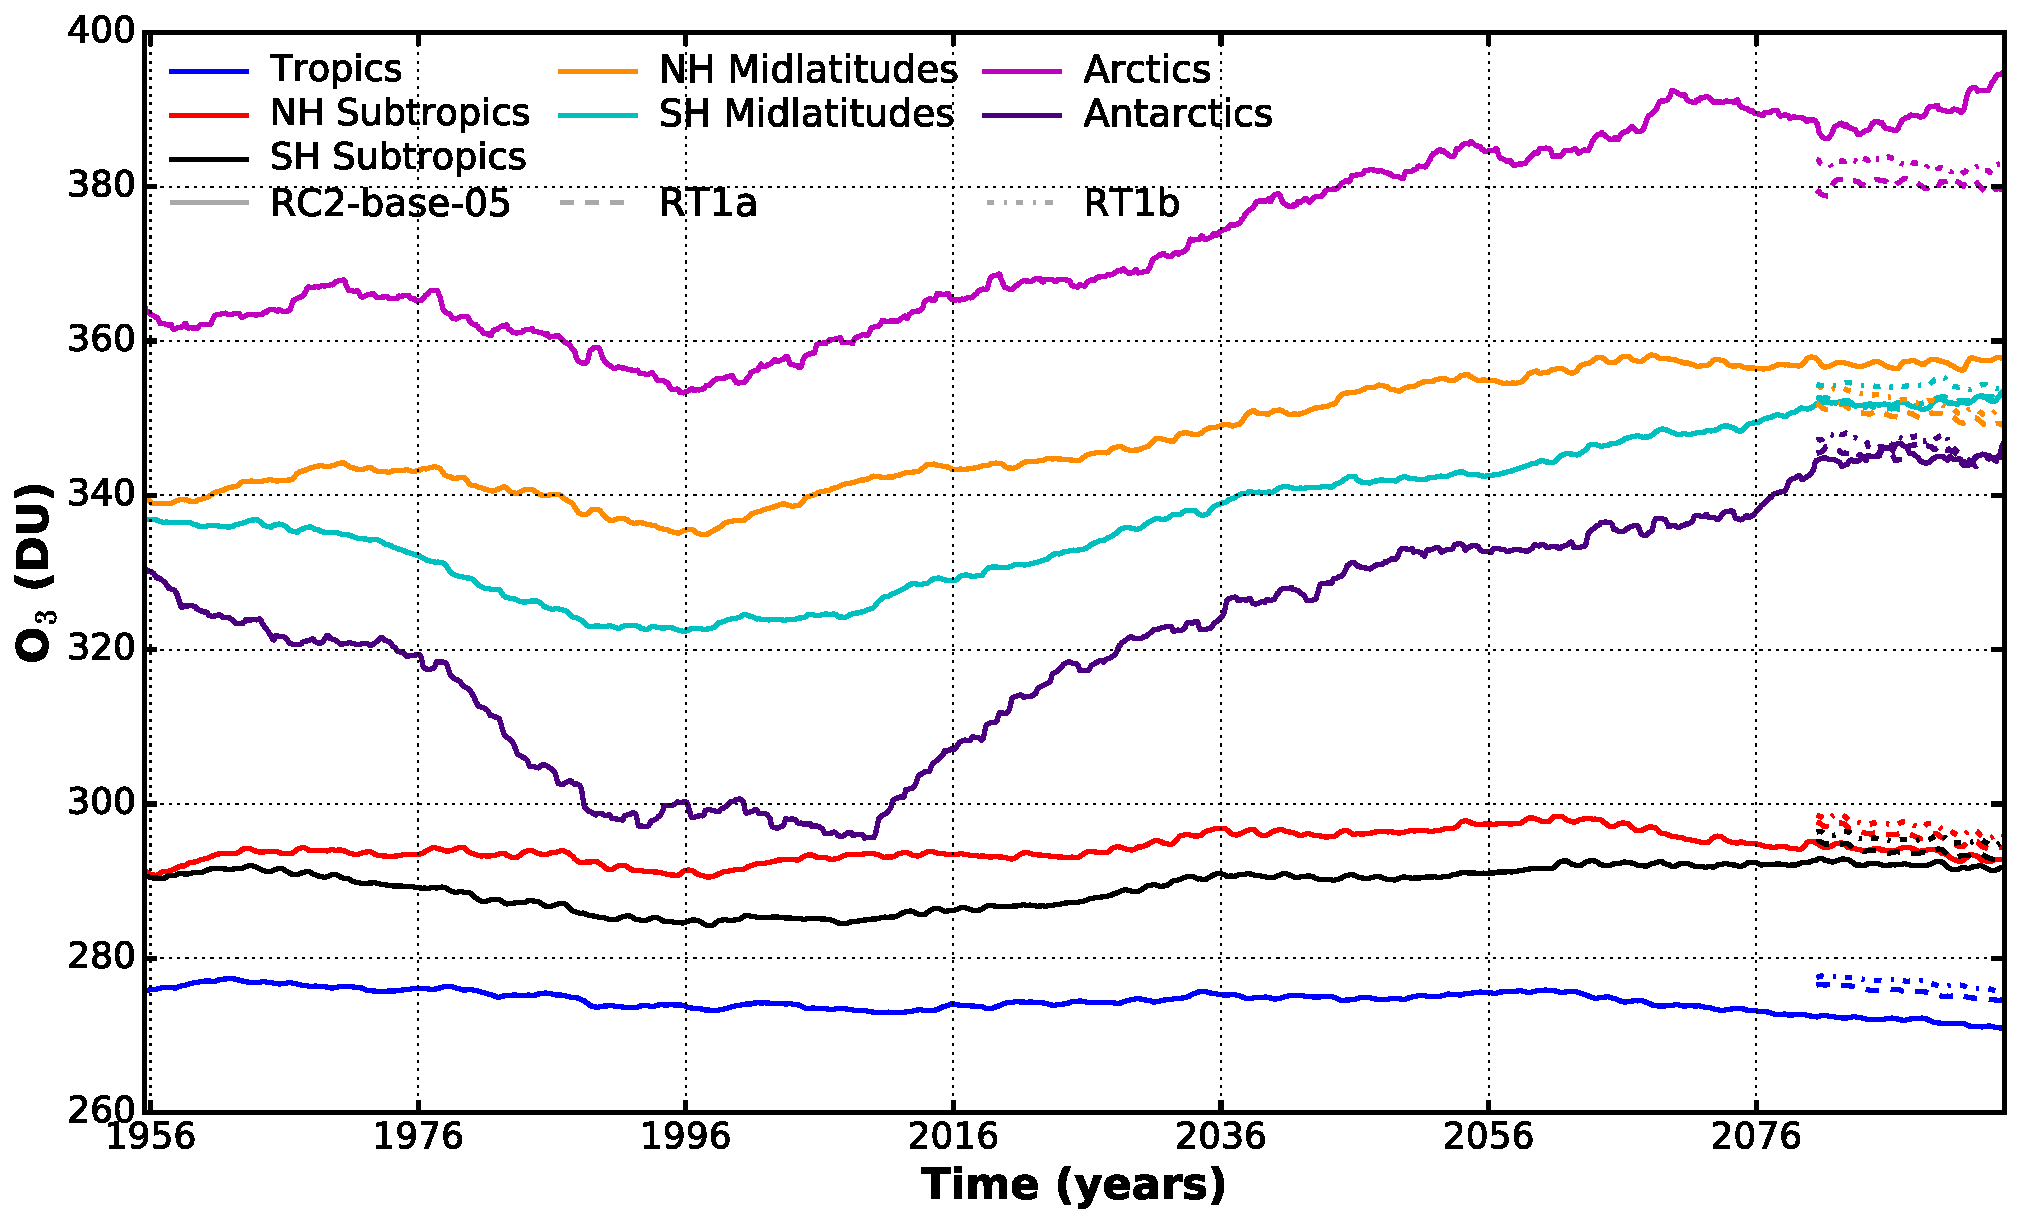
\includegraphics[width=8.3cm]{fig10}
  \caption{Zonal mean ozone trend from RC2-base-05 (1950--2100) and RT1a/RT1b (2080--2100). Smoothed with moving average box window 11 years.}
  \label{fig:Zonal_Total_Ozone}
\end{figure}
%
\begin{figure*}[t]
  \centering
  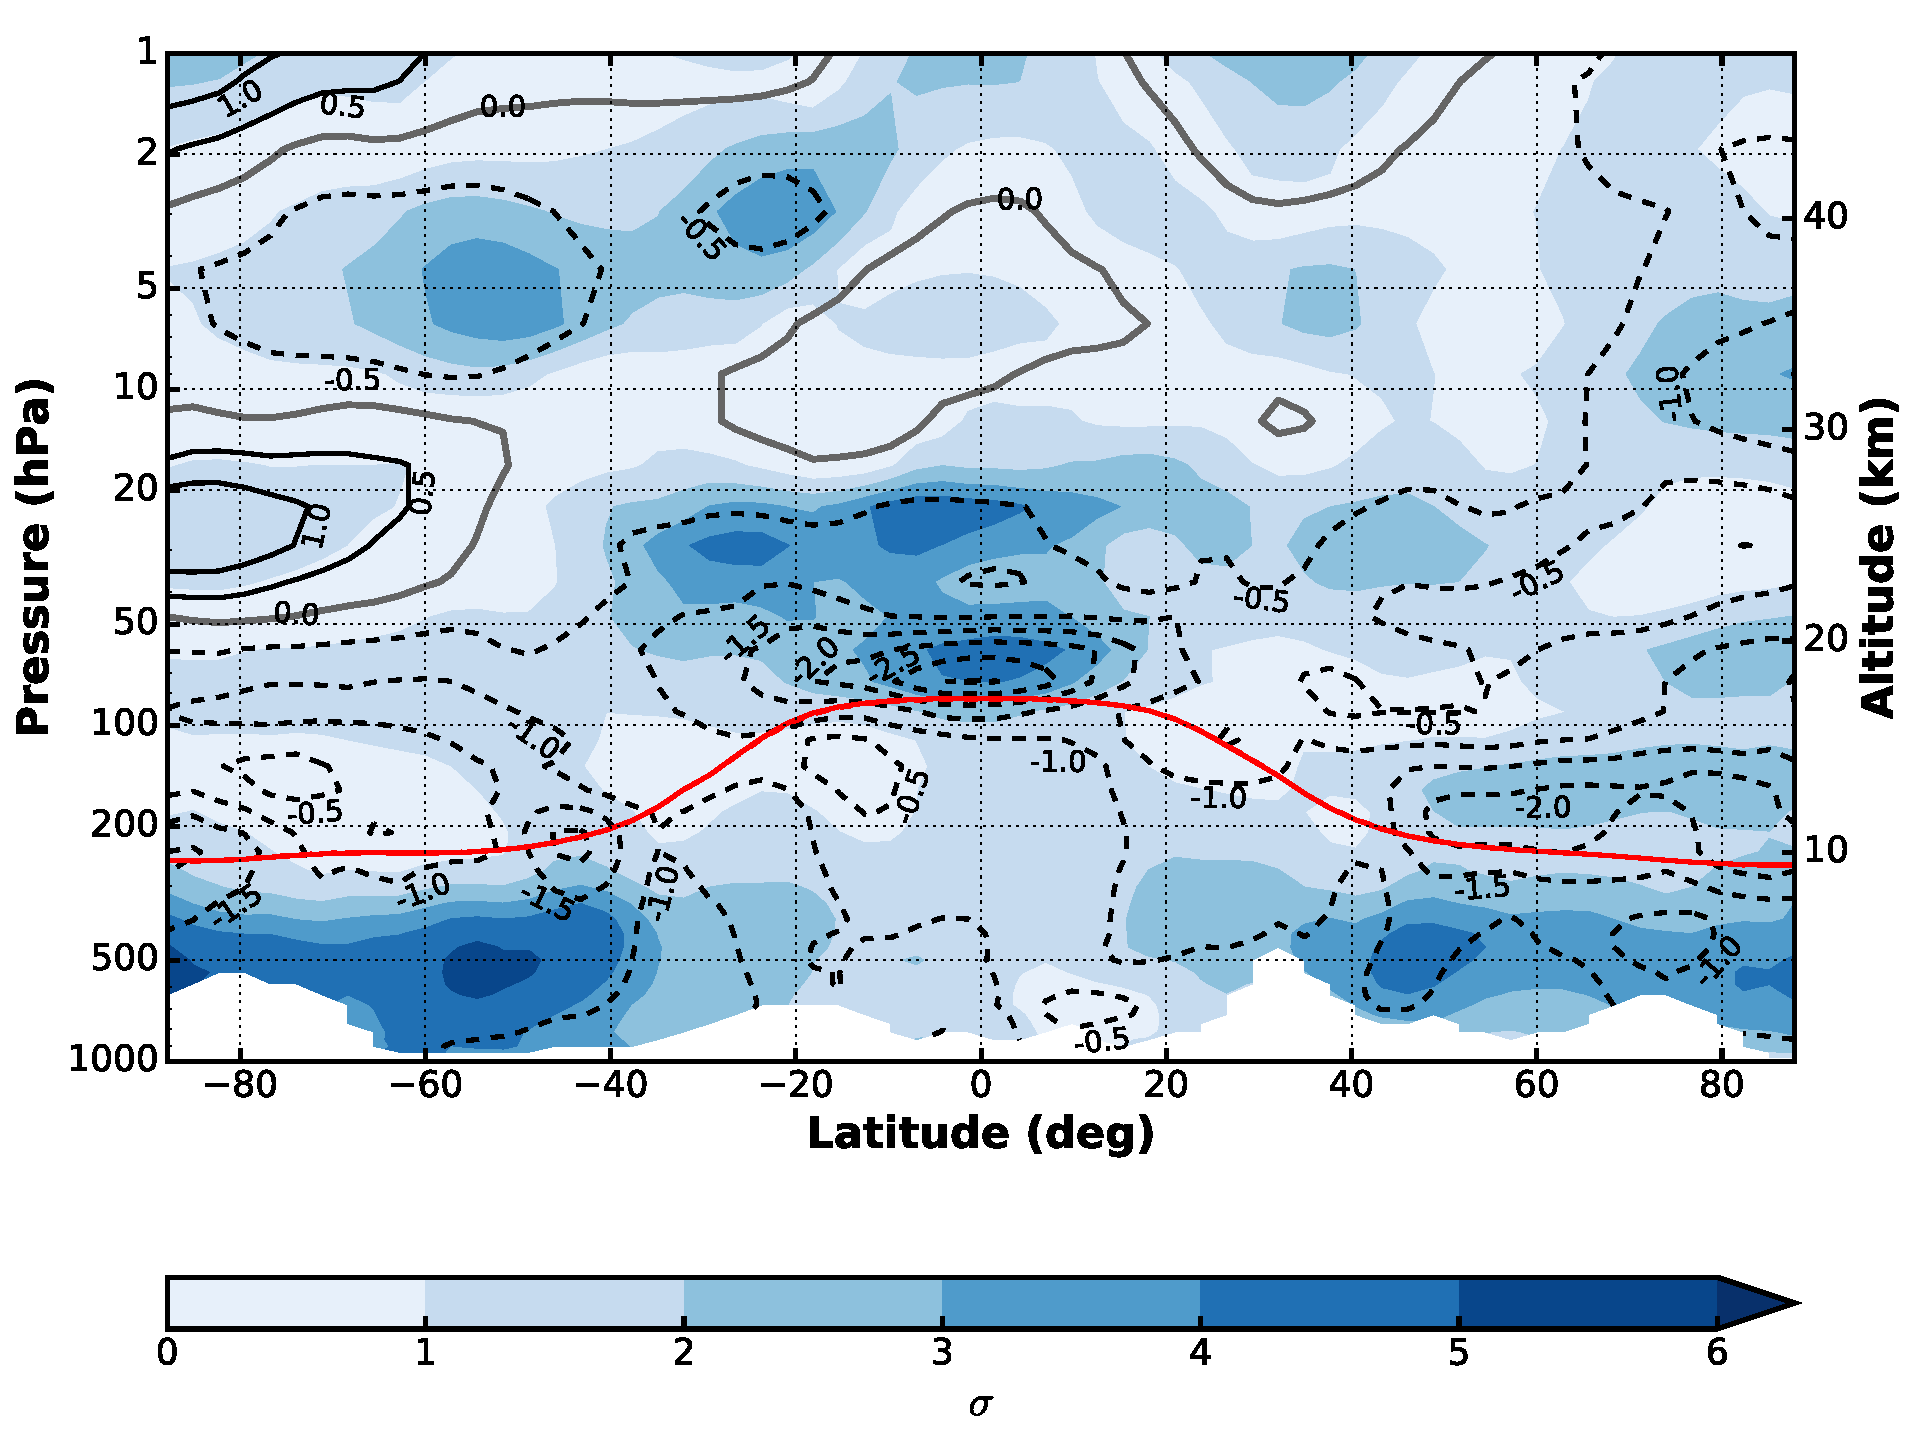
\includegraphics[width=12cm]{fig11}
  \caption{Ozone reduction due to VSLS. Medium-term full-chemistry future simulation with and without VSLS. Zonal mean profile of decadal mean difference in percent ($\mathrm{(RT1a-RT1b)/RT1a\cdot100}$). Dashed lines indicate a decrease of ozone in the simulation with VSLS turned on (RT1a) compared to the one with VSLS turned off (RT1b). The average tropopause is shown as red line. Significance is indicated by blue shaded areas. The significance is estimated as manifold of difference from zero in units of standard error of mean difference.}
  \label{fig:zonal_mean_ozone}
\end{figure*}
%
\conclusions  %% \conclusions[modified heading if necessary]
\label{sec:conclusion}
We have investigated long-term changes in emission and transport of brominated VSLS under a changing climate (RCP6.0). Under the implicit assumption of constant concentrations of VSLS in the ocean waters, over a time-span of 120 years, we have found an enhancement of zonally averaged fluxes of \chem{CH_2Br_2} and \chem{CHBr_3} in the order of 10\% between present day and the end of the 21st century. A strong increase of flux (up to 55\% in \chem{CH_2Br_2} and 25\% in \chem{CHBr_3}) has been found in the northern hemisphere polar region. There, the retreat of sea ice is playing a key role. Exposing almost the entire polar ocean in August--September by the end of the 21st century, sea ice does not longer act as a lid to ocean--atmosphere fluxes of VSLS. Sea ice itself has not been considered a source of VSLS in our simulations. \DIFdelbegin \DIFdel{The subsequent }\DIFdelend \DIFaddbegin \DIFadd{Subsequently, an }\DIFaddend increase of organic bromine in the UTLS is \DIFaddbegin \DIFadd{found }\DIFaddend of the same order of magnitude (8--10\%).\\
%
\DIFdelbegin \DIFdel{Since ocean--atmosphere }\DIFdelend \DIFaddbegin \DIFadd{Ocean--atmosphere }\DIFaddend fluxes are sensitive to the abundance of VSLS in the atmosphere \DIFdelbegin \DIFdel{, an }\DIFdelend \DIFaddbegin \DIFadd{as well as on wind speed. An }\DIFaddend increased dissociation of VSLS in the lowermost troposphere, e.g., due to increasing \chem{OH} concentrations in the RCP6.0 scenario, reduces the atmospheric concentration and therefore increases the flux from the ocean to the atmosphere without necessarily increasing the actual amount which is transported to the stratosphere. \DIFaddbegin \DIFadd{The total amount of bromine from VSLS transported through the UTLS strongly depends on the washout of inorganic PG (}\chem{Br_y^{VSLS}}\DIFadd{) and hence on the partitioning and heterogeneous reactions converting }\chem{Br_y^{VSLS}} \DIFadd{between soluble, e.g., }\chem{HBr}\DIFadd{, }\chem{HOBr}\DIFadd{, and insoluble, e.g., }\chem{BrO}\DIFadd{, species. But these mechanisms have not been subject to our study.}\DIFaddend \\
%
\DIFdelbegin \DIFdel{Assuming a constant, prescribed flux of VSLS over the course of 150 years, we have developed a simple, analytic ansatz to disentangled various factors affecting the future abundance of bromine from VSLS in the atmosphere.All occurring future changes in temperature, }%DIFDELCMD < [\chem{OH}]%%%
\DIFdel{, AOA, and photolysis frequency decrease the VMR of VSLS in the troposphere (in total $\sim$5--10\%).In case of }%DIFDELCMD < \chem{CHBr_3}%%%
\DIFdel{, all factors listed are of the same order of magnitude. The tropospheric decrease of }%DIFDELCMD < \chem{CH_2Br_2} %%%
\DIFdel{VMR is mainly driven by increasing }%DIFDELCMD < [\chem{OH}]%%%
\DIFdel{.In the UTLS, the impact of rejuvenating AOA dominates, inflicting an increase in VSLS VMR in the order of }\DIFdelend \DIFaddbegin \DIFadd{For prescribed, constant VSLS fluxes, an increase of lower stratospheric VSLS of about }\DIFaddend 5--10\% \DIFdelbegin \DIFdel{. In general, the features of the actual difference profiles are well reproduced by our ansatz. The effect of AOA on }%DIFDELCMD < \chem{CH_2Br_2} %%%
\DIFdel{is, however, slightly overestimated.}%DIFDELCMD < \\
%DIFDELCMD < %%%
%DIF < 
\DIFdel{Due to the rise of the tropical tropopause by 0.81}\DIFdelend \DIFaddbegin \DIFadd{is due to enhanced vertical transport in the tropics. This increase is counteracted by a corresponding decrease in inorganic bromine. Everything else unchanged, an increase in tropical upwelling will not change the total amount of bromine in the future stratosphere. Additionally, due to enhanced future }\chem{OH} \DIFadd{concentrations in the RCP6.0 emission scenario, the tropospheric lifetime of VSLS is reduced, which leads to a decrease of total bromine from VSLS. Furthermore we have diagnosed a decrease of }\chem{Br_{tot}^{VSLS}} \DIFadd{by 0.5--2}\DIFaddend \,\DIFdelbegin %DIFDELCMD < \unit{hPa\,decade^{-1}}%%%
\DIFdel{, air which at present is considered stratospheric will be still tropospheric in the future. If taken into account by shifting VSLS VMR profiles }\DIFdelend \DIFaddbegin \unit{ppt} \DIFadd{for a fixed pressure level }\DIFaddend with respect to the mean \DIFdelbegin \DIFdel{model tropopause height, }\DIFdelend \DIFaddbegin \DIFadd{tropical tropopause $\Delta_\mathrm{TP}P \approx 20$\,}\unit{hPa}\DIFadd{, if the upward shift of }\DIFaddend the \DIFdelbegin \DIFdel{total amount of bromine in the tropical UTLS is decreasing by roughly 2}\DIFdelend \DIFaddbegin \DIFadd{mean tropical tropopause of $(0.81)$}\DIFaddend \,\DIFdelbegin %DIFDELCMD < \unit{ppt}%%%
\DIFdel{. Overall, the amount of bromine in the UTLS is decreasing in this future scenario}\DIFdelend \DIFaddbegin \unit{hPa\,decade^{-1}} \DIFadd{is taken into consideration}\DIFaddend .\\
%
The impact of enhanced fluxes of brominated VSLS on future ozone abundance has been evaluated by comparing two experiments of which one has no VSLS emission and the other interactively computed fluxes from constant ocean concentrations of VSLS. We have found a significant reduction of ozone in the tropical UTLS of about 3\%. In the troposphere the largest significant decrease of ozone amounts to 1--2\%. Thus, bromine from VSLS may not act as a major source to future stratospheric ozone depletion.
%
While interactive emissions from constant ocean concentrations \DIFdelbegin \DIFdel{and aerosol formation }\DIFdelend have been taken into consideration, the actual climate change inflicted change in the production of VSLS by macroalgae in the ocean remains an open question. Whether the found increase of ocean--atmosphere fluxes of VSLS and a future decrease of VSLS in the troposphere will cancel out or overcompensate would need further simulation studies.
%
%DIF < \section{Code availability}
%DIF < TEXT
\section{\DIFdelbegin \DIFdel{Data }\DIFdelend \DIFaddbegin \DIFadd{Code }\DIFaddend availability}
The Modular Earth Submodel System (MESSy) is continuously further developed and applied by a consortium of institutions. The usage of MESSy and access to the source code is licensed to all affiliates of institutions, which are members of the MESSy Consortium. Institutions can become a member of the MESSy Consortium by signing the MESSy Memorandum of Understanding. More information can be found on the MESSy Consortium Web-site (\url{http://www.messy-interface.org}).
\DIFdelbegin %DIFDELCMD < \\
%DIFDELCMD < %%%
\DIFdelend \DIFaddbegin \section{\DIFadd{Data availability}}
\DIFaddend The data of the ESCiMo simulations will be made available in the Climate and Environmental Retrieval and Archive (CERA) database at the German Climate Computing Centre (DKRZ; \url{http://cera-www.dkrz.de/WDCC/ui/Index.jsp}). The corresponding digital object identifiers (doi) will be published on the MESSy consortium web-page (\url{http://www.messy-interface.org}). A subset of the data of those simulations covering consistently the requested time periods (1960--2010 for RC1, and 1960--2099 for RC2) will be submitted to the BADC database for the CCMI project.\\
Data from ROMIC--THREAT associated simulations (RT1a, RT1b) and simplified chemistry (SC\_free, SC\_nudged) will be made available on request.
%\appendix
%\section{}    %% Appendix A

%\subsection{}     %% Appendix A1, A2, etc.

%\appendixfigures  %% needs to be added in front of appendix figures in one-column style (\documentclass[acp, manuscript]{copernicus})

%\appendixtables   %% needs to be added in front of appendix tables in one-column style (\documentclass[acp, manuscript]{copernicus})

\authorcontribution{S. Falk performed most of the analyses and wrote the paper. B.-M. Sinnhuber conceived this study and provided advice through discussion of the analysis and results. G. Krysztofiak developed and performed the simplified chemistry simulations as well as part of the corresponding data analysis in Sec.~\ref{sec:emission_trends}. S.~T. Lennatz provided advise on the ocean--atmosphere gas exchange. P. J\"{o}ckel provided advice as project leader of the ESCiMo consortial project and coordinator of overall EMAC model development; preparation of the ESCiMo model setups and realization of the ESCiMo simulations of ESCiMo consortium, with VSLS boundary conditions and implementation of the online \chem{Br} budget diagnostics for EMAC prepared by P. Graf. All coauthors contributed to the discussion of the results.}

\competinginterests{The authors declare that they have no conflict of interest.}

%\disclaimer{TEXT}

\begin{acknowledgements}
Parts of this work were supported by the Deutsche Forschungsgemeinschaft (DFG) through the research unit 'SHARP' (SI1044/1-2), the German Bundesministerium f\"{u}r Bildung und Forschung (BMBF) through the project 'ROMIC-THREAT' (01GL1217B), the European Union through the Horizon 2020 project 'GAIA-CLIM', and by the Helmholtz Association through its research program 'ATMO'.\\
The CNRM data were produced in the framework of the CCMI project, with support of M\'{e}t\'{e}o--France. We particularly acknowledge the support of M. Michou and D. Saint--Martin and of the entire team in charge of the CNRM/CERFACS climate model.\\
NOAA Optimum Interpolation~(OI)~V2 fields were provided by the National Centers for Environmental Prediction/National Weather Service/NOAA/U.S. Department of Commerce, and National Climatic Data Center/NESDIS/NOAA/U.S. Department of Commerce research Data Archive at the National Center for Atmospheric Research, Computational and Information Systems Laboratory. \url{http://rda.ucar.edu/datasets/ds277.0/}. Accessed 06 January 2016).\\
The ESCiMo (Earth System Chemistry integrated Modelling) model simulations have been performed at the German Climate Computing Centre~(DKRZ) through support from the BMBF. DKRZ and its scientific steering committee are gratefully acknowledged for providing the HPC and data archiving resources for this consortial project.\\
EMAC simulations RT1a/1b have been performed at Steinbuch Center for Computing at KIT. Thanks to Stefan Versick and Oliver Kirner (KIT SimLab Climate and Environment) for their technical support.\\
Special thanks to C. Br\"{u}hl (MPI-Mainz) for his help in implementing additional sulfur reactions and usage of \texttt{gmxe} in context of the ROMIC--THREAT simulations.\\
S. Lennartz likes to thank B. Quack, C. Marandino, S. Tegtmeier (all Helmholtz-Centre for Ocean Research Kiel), and K. Kr\"{u}ger (University of Oslo) for their support.
\end{acknowledgements}

%% REFERENCES
%% Since the Copernicus LaTeX package includes the BibTeX style file copernicus.bst,
%% authors experienced with BibTeX only have to include the following two lines:
%%
\bibliographystyle{copernicus}
\bibliography{vsls_emissions}
%%
%% URLs and DOIs can be entered in your BibTeX file as:
%%
%% URL = {http://www.xyz.org/~jones/idx_g.htm}
%% DOI = {10.5194/xyz}

%% LITERATURE CITATIONS
%%
%% command                        & example result
%% \citet{jones90}|               & Jones et al. (1990)
%% \citep{jones90}|               & (Jones et al., 1990)
%% \citep{jones90,jones93}|       & (Jones et al., 1990, 1993)
%% \citep[p.~32]{jones90}|        & (Jones et al., 1990, p.~32)
%% \citep[e.g.,][]{jones90}|      & (e.g., Jones et al., 1990)
%% \citep[e.g.,][p.~32]{jones90}| & (e.g., Jones et al., 1990, p.~32)
%% \citeauthor{jones90}|          & Jones et al.
%% \citeyear{jones90}|            & 1990

%% FIGURES

%% We suggest to put the figures in the correct order and placement within the text. This aids readability.
%% When figures and tables are placed at the end of the MS (article in one-column style), please add \clearpage
%% between bibliography and first table and/or figure as well as between each table and/or figure.

%% ONE-COLUMN FIGURES
%%f
%\begin{figure}[t]
%\includegraphics[width=8.3cm]{FILE NAME}
%\caption{TEXT}
%\end{figure}
%
%%% TWO-COLUMN FIGURES
%
%%f
%\begin{figure*}[t]
%\includegraphics[width=12cm]{FILE NAME}
%\caption{TEXT}
%\end{figure*}
%
%
%%% TABLES
%%%
%%% The different columns must be seperated with a & command and should
%%% end with \\ to identify the column brake.
%
%%% ONE-COLUMN TABLE
%
%%t
%\begin{table}[t]
%\caption{TEXT}
%\begin{tabular}{column = lcr}
%\tophline
%
%\middlehline
%
%\bottomhline
%\end{tabular}
%\belowtable{} % Table Footnotes
%\end{table}
%
%%% TWO-COLUMN TABLE
%
%%t
%\begin{table*}[t]
%\caption{TEXT}
%\begin{tabular}{column = lcr}
%\tophline
%
%\middlehline
%
%\bottomhline
%\end{tabular}
%\belowtable{} % Table Footnotes
%\end{table*}
%
%
%%% MATHEMATICAL EXPRESSIONS
%
%%% All papers typeset by Copernicus Publications follow the math typesetting regulations
%%% given by the IUPAC Green Book (IUPAC: Quantities, Units and Symbols in Physical Chemistry,
%%% 2nd Edn., Blackwell Science, available at: http://old.iupac.org/publications/books/gbook/green_book_2ed.pdf, 1993).
%%%
%%% Physical quantities/variables are typeset in italic font (t for time, T for Temperature)
%%% Indices which are not defined are typeset in italic font (x, y, z, a, b, c)
%%% Items/objects which are defined are typeset in roman font (Car A, Car B)
%%% Descriptions/specifications which are defined by itself are typeset in roman font (abs, rel, ref, tot, net, ice)
%%% Abbreviations from 2 letters are typeset in roman font (RH, LAI)
%%% Vectors are identified in bold italic font using \vec{x}
%%% Matrices are identified in bold roman font
%%% Multiplication signs are typeset using the LaTeX commands \times (for vector products, grids, and exponential notations) or \cdot
%%% The character * should not be applied as mutliplication sign
%
%
%%% EQUATIONS
%
%%% Single-row equation
%
%\begin{equation}
%
%\end{equation}
%
%%% Multiline equation
%
%\begin{align}
%& 3 + 5 = 8\\
%& 3 + 5 = 8\\
%& 3 + 5 = 8
%\end{align}
%
%
%%% MATRICES
%
%\begin{matrix}
%x & y & z\\
%x & y & z\\
%x & y & z\\
%\end{matrix}
%
%
%%% ALGORITHM
%
%\begin{algorithm}
%\caption{�}
%\label{a1}
%\begin{algorithmic}
%�
%\end{algorithmic}
%\end{algorithm}
%
%
%%% CHEMICAL FORMULAS AND REACTIONS
%
%%% For formulas embedded in the text, please use \chem{}
%
%%% The reaction environment creates labels including the letter R, i.e. (R1), (R2), etc.
%
%\begin{reaction}
%%% \rightarrow should be used for normal (one-way) chemical reactions
%%% \rightleftharpoons should be used for equilibria
%%% \leftrightarrow should be used for resonance structures
%\end{reaction}
%
%
%%% PHYSICAL UNITS
%%%
%%% Please use \unit{} and apply the exponential notation


\end{document}
